\clearpage \documentclass[a4paper,12pt,notitlepage]{article}

\frenchspacing
\usepackage{a4}
\usepackage[pdftitle={Vypracovane otazky k bakalarskym statnicim}, pdfauthor={študenti MFF}, pdfdisplaydoctitle=true, colorlinks=false,unicode=true,pdfborder=0 0 0]{hyperref}
\usepackage{slovak}
\usepackage{ucs}
\usepackage[utf8x]{inputenc}

\title{Vypracovane otazky k bakalarskym statnicim}
\author{študenti MFF}

\usepackage{graphicx}
\usepackage{amsmath,amssymb,amsthm}
\usepackage{color}
\usepackage[left=3cm, right=3cm, top=3cm, bottom=3cm]{geometry} % nastavení dané velikosti okrajů


%Vacsina prostredi je dvojjazicne. V pripade, ze znenie napr pozorovania je pisane po slovensky, malo by byt po slovensky aj oznacenie.

\newenvironment{pozadavky}{\pagebreak[2]\noindent\textbf{Požadavky}\par\noindent\leftskip 10pt}{\par\bigskip}
\newenvironment{poziadavky}{\pagebreak[2]\noindent\textbf{Požiadavky}\par\noindent\leftskip 10pt}{\par\bigskip}

\newenvironment{definice}{\pagebreak[2]\noindent\textbf{Definice}\par\noindent\leftskip 10pt}{\par\bigskip}
\newenvironment{definiceN}[1]{\pagebreak[2]\noindent\textbf{Definice~}\emph{(#1)}\par\noindent\leftskip 10pt}{\par\bigskip}
\newenvironment{definicia}{\pagebreak[2]\noindent\textbf{Definícia}\par \noindent\leftskip 10pt}{\par\bigskip}
\newenvironment{definiciaN}[1]{\pagebreak[2]\noindent\textbf{Definícia~}\emph{(#1)}\par\noindent\leftskip 10pt}{\par\bigskip}

\newenvironment{pozorovani}{\pagebreak[2]\noindent\textbf{Pozorování}\par\noindent\leftskip 10pt}{\par\bigskip}
\newenvironment{pozorovanie}{\pagebreak[2]\noindent\textbf{Pozorovanie}\par\noindent\leftskip 10pt}{\par\bigskip}
\newenvironment{poznamka}{\pagebreak[2]\noindent\textbf{Poznámka}\par\noindent\leftskip 10pt}{\par\bigskip}
\newenvironment{poznamkaN}[1]{\pagebreak[2]\noindent\textbf{Poznámka~}\emph{(#1)}\par\noindent\leftskip 10pt}{\par\bigskip}
\newenvironment{lemma}{\pagebreak[2]\noindent\textbf{Lemma}\par\noindent\leftskip 10pt}{\par\bigskip}
\newenvironment{lemmaN}[1]{\pagebreak[2]\noindent\textbf{Lemma~}\emph{(#1)}\par\noindent\leftskip 10pt}{\par\bigskip}
\newenvironment{veta}{\pagebreak[2]\noindent\textbf{Věta}\par\noindent\leftskip 10pt}{\par\bigskip}
\newenvironment{vetaN}[1]{\pagebreak[2]\noindent\textbf{Věta~}\emph{(#1)}\par\noindent\leftskip 10pt}{\par\bigskip}
\newenvironment{vetaSK}{\pagebreak[2]\noindent\textbf{Veta}\par\noindent\leftskip 10pt}{\par\bigskip}
\newenvironment{vetaSKN}[1]{\pagebreak[2]\noindent\textbf{Veta~}\emph{(#1)}\par\noindent\leftskip 10pt}{\par\bigskip}

\newenvironment{dusledek}{\pagebreak[2]\noindent\textbf{Důsledek}\par\noindent\leftskip 10pt}{\par\bigskip}
\newenvironment{dosledok}{\pagebreak[2]\noindent\textbf{Dôsledok}\par\noindent\leftskip 10pt}{\par\bigskip}

\newenvironment{dokaz}{\pagebreak[2]\noindent\leftskip 10pt\textbf{Dôkaz}\par\noindent\leftskip 10pt}{\par\bigskip}
\newenvironment{dukaz}{\pagebreak[2]\noindent\leftskip 10pt\textbf{Důkaz}\par\noindent\leftskip 10pt}{\par\bigskip}

\newenvironment{priklad}{\pagebreak[2]\noindent\textbf{Příklad}\par\noindent\leftskip 10pt}{\par\bigskip}
\newenvironment{prikladSK}{\pagebreak[2]\noindent\textbf{Príklad}\par\noindent\leftskip 10pt}{\par\bigskip}
\newenvironment{priklady}{\pagebreak[2]\noindent\textbf{Příklady}\par\noindent\leftskip 10pt}{\par\bigskip}
\newenvironment{prikladySK}{\pagebreak[2]\noindent\textbf{Príklady}\par\noindent\leftskip 10pt}{\par\bigskip}

\newenvironment{algoritmusN}[1]{\pagebreak[2]\noindent\textbf{Algoritmus~}\emph{(#1)}\par\noindent\leftskip 10pt}{\par\bigskip}
%obecne prostredie, ktore ma vyuzitie pri specialnych odstavcoch ako (uloha, algoritmus...) aby nevzniklo dalsich x prostredi
\newenvironment{obecne}[1]{\pagebreak[2]\noindent\textbf{#1}\par\noindent\leftskip 10pt}{\par\bigskip}


\newenvironment{penumerate}{
\begin{enumerate}
  \setlength{\itemsep}{1pt}
  \setlength{\parskip}{0pt}
  \setlength{\parsep}{0pt}
  %\setlength{\topsep}{200pt}
  \setlength{\partopsep}{200pt}
}{\end{enumerate}}

\def\pismenka{\numberedlistdepth=2} %pouzit, ked clovek chce opismenkovany zoznam...

\newenvironment{pitemize}{
\begin{itemize}
  \setlength{\itemsep}{1pt}
  \setlength{\parskip}{0pt}
  \setlength{\parsep}{0pt}
}{\end{itemize}}

\definecolor{gris}{gray}{0.95}
\newcommand{\ramcek}[2]{\begin{center}\fcolorbox{white}{gris}{\parbox{#1}{#2}}\end{center}\par}
 \clearpage
\title{\LARGE Učební texty k státní bakalářské zkoušce \\ Programování \\ Databáze}
\begin{document}
\maketitle
\newpage
\setcounter{section}{2}
\section{Databáze}
\begin{pozadavky}
\begin{pitemize}
\item Podstata a architektury DB systémů
\item Konceptuální, logická a fyzická úroveň pohledů na data
\item Algoritmy návrhu schémat relací, normální formy, referenční integrita
\item Transakční zpracování, vlastnosti transakcí, uzamykací protokoly, zablokování
\item ER-diagramy, metody návrhů IS
\item SQL
\item Indexy, triggery, uložené procedury, uživatelé, uživatelská práva
\item Vícevrstevné architektury
\item Vazba databází na internetové technologie
\item Organizace dat na vnější paměti, B-stromy a jejich varianty.
\end{pitemize}
\end{pozadavky}
\subsection{Podstata a architektury DB systemů}

Zdroje: Wikipedie, slidy Dr. T. Skopala k Databázovým systémům
\bigskip

\begin{definiceN}{Databáze}
Databáze je logicky uspořádaná (integrovaná) kolekce navzájem souvisejících dat. Je sebevysvětlující, protože data jsou uchovávána společně s popisy, známými jako metadata (také schéma databáze). Data jsou ukládána tak, aby na nich bylo možné provádět strojové dotazy -- získat pro nějaké parametry vyhovující podmnožinu záznamů.

Někdy se slovem \uv{databáze} myslí obecně celý databázový systém.
\end{definiceN}

\begin{definiceN}{Systém řízení báze dat}
Systém řízení báze dat (SŘBD, anglicky database management system, DBMS) je obecný softwarový systém, který řídí sdílený přístup k databázi, a poskytuje mechanismy, pomáhající zajistit bezpečnost a integritu uložených dat. Spravuje databázi a zajišťuje provádění dotazů.
\end{definiceN}

\begin{definiceN}{Databázový systém}
Databázovým systémem rozumíme trojici, sestávající z:
\begin{pitemize}
    \item databáze
    \item systému řízení báze dat
    \item chudáka admina
\end{pitemize}
\end{definiceN}

\begin{obecne}{Smysl databází}
Hlavním smyslem databáze je schraňovat datové záznamy a informace za účelem:
\begin{pitemize}
    \item sdílení dat více uživateli,
    \item zajištění unifikovaného rozhraní a jazyků definice dat a manipulace s daty,
    \item znovuvyužitelnosti dat,
    \item bezespornosti dat a
    \item snížení objemu dat (odstranění redundance).
\end{pitemize}
\end{obecne}

\subsubsection*{Databázové modely}

\begin{definiceN}{schéma, model}
Typicky pro každou databázi existuje strukturální popis druhů dat v ní udržovaných, ten nazýváme \emph{schéma}. Schéma popisuje objekty reprezentované v databázi a vztahy mezi nimi. Je několik možných způsobů organizace schémat (modelování databázové struktury), známých jako \emph{modely}. V modelu jde nejen o způsob strukturování dat, definuje se také sada operací nad daty proveditelná. Relační model například definuje operace jako \uv{select} nebo \uv{join}. I když tyto operace se nemusejí přímo vyskytovat v dotazovacím jazyce, tvoří základ, na kterém je jazyk postaven. Nejdůležitější modely v této sekci popíšeme.
\end{definiceN}

\begin{poznamka}
Většina databázových systémů je založena na jednom konkrétním modelu, ale čím dál častější je podpora více přístupů. Pro každý logický model existuje více fyzických přístupů implementace a většina systémů dovolí uživateli nějakou úroveň jejich kontroly a úprav, protože toto má velký vliv na výkon systému. Příkladem nechť jsou indexy, provozované nad relačním modelem.
\end{poznamka}

\begin{obecne}{\uv{Plochý} model}
Toto sice nevyhovuje úplně definici modelu, přesto se jako triviální případ uvádí. Představuje jedinou dvoudimensionální tabulku, kde data v jednom sloupci jsou považována za popis stejné vlastnosti (takže mají podobné hodnoty) a data v jednom řádku se uvažují jako popis jediného objektu.
\end{obecne}

\begin{obecne}{Relační model}
Relační model je založen na predikátové logice a teorii množin. Většina fyzicky implementovaných databázových systémů ve skutečnosti používá jen aproximaci matematicky definovaného relačního modelu. Jeho základem jsou \emph{relace} (dvoudimensionální tabulky), \emph{atributy} (jejich pojmenované sloupce) a \emph{domény} (množiny hodnot, které se ve sloupcích můžou objevit). Hlavní datovou strukturou je tabulka, kde se nachází informace o nějaké konkrétní  třídě entit. Každá entita té třídy je potom reprezentována řádkem v tabulce -- $n$-ticí atributů.

Všechny relace (tj. tabulky) musí splňovat základní pravidla -- pořadí sloupců nesmí hrát roli, v tabulce se nesmí vyskytovat identické řádky a každý řádek musí obsahovat jen jednu hodnotu pro každý svůj atribut. Relační databáze obsahuje více tabulek, mezi kterými lze popisovat vztahy (všech různých kardinalit, tj. $1:1$, $1:n$ apod.). Vztahy vznikají i implicitně např. uložením stejné hodnoty jednoho atributu do dvou řádků v tabulce. K tabulkám lze přidat informaci o tom, která podmnožina atributů funguje jako \emph{klíč}, tj. unikátně identifikuje každý řádek, některý z klíčů může být označen jako primární. Některé klíče můžou mít nějaký vztah k vnějšímu světu, jiné jsou jen pro vnitřní potřeby schématu databáze (generovaná ID).
\end{obecne}

\begin{obecne}{Hierarchický model}
V hierarchickém modelu jsou data organizována do stromové struktury -- každý uzel má odkaz na nadřízený (k popisu hierarchie) a setříděné pole záznamů na stejné úrovni. Tyto struktury byly používány ve starých mainframeových databázích, nyní je můžeme vidět např ve struktuře XML dokumentů. Dovolují vztahy $1:N$ mezi dvěma druhy dat, což je velice efektivní k popisu různých reálných vztahů (obsahy, řazení odstavců textu, tříděné informace). Nevýhodou je ale nutnost znát celou cestu k záznamu ve struktuře a neschopnost systému reprezentovat redundance v datech (strom nemá cykly).
\end{obecne}

\begin{obecne}{Síťový model}
Síťový model organizuje data pomocí dvou hlavních prvků, \emph{záznamů} a \emph{množin}. Záznamy obsahují pole dat, množiny definují vztahy $1:N$ mezi záznamy (jeden \emph{vlastník}, mnoho \emph{prvků}). Záznam může být vlastníkem i prvkem v několika různých množinách. Jde vlastně o variantu hierarchického modelu, protože síťový model je také založen na konceptu více struktur nižší úrovně závislých na strukturách úrovně vyšší. Už ale umožňuje reprezentovat i redundantní data. Operace nad tímto modelem probíhají \uv{navigačním} stylem: program si uchovává svoji současnou pozici mezi záznamy a postupuje podle závislostí, ve kterých se daný záznam náchází. Záznamy mohou být i vyhledávány podle klíče. 

Fyzicky jsou většinou množiny -- vztahy -- reprezentovány přímo ukazateli na umístění dat na disku, což zajišťuje vysoký výkon při vyhledávání, ale zvyšuje náklady na reorganizace. Smysl síťové navigace mezi objekty se používá i v objektových modelech.
\end{obecne}

\begin{obecne}{Objektový model}
Objektový model je aplikací přístupů známých z objektově-orientovaného programování. Je založen na sbližování programové aplikace a databáze, hlavně ve smyslu použití datových typů (objektů) definovaných na jednom místě; ty zpřístupňuje k použití v nějakém běžném programovacím jazyce. Odstraní se tak nutnost zbytečných konverzí dat. Přináší do databází také věci jako zapouzdření nebo polymorfismus. Problémem objektových modelů je neexistence standardů (nebo spíš produktů, které by je implementovaly).

Kombinací objektového a relačního přístupu vznikají \emph{objektově-relační} databáze -- relační databáze, dovolující uživateli definovat vlastní datové typy a operace na nich. Obsahují pak hybrid mezi procedurálním a dotazovacím programovacím jazykem.

\end{obecne}


\subsubsection*{Architektury databázových systémů}

Zdroj: Wiki ČVUT (státnice na FELu ;-))
\bigskip

Architektury databázových systémů se obecně dělí na 
\begin{pitemize}
    \item \emph{centralizované} (kde se databáze předpokládá fyzicky na jednom počítači) a
    \item \emph{distribuované},
\end{pitemize}
případně na
\begin{pitemize}
    \item \emph{jednouživatelské} a
    \item \emph{víceuživatelské}.
\end{pitemize}

\begin{obecne}{Distribuované databázové systémy}
\emph{Distribuovaný systém řízení báze dat} je vlastně speciálním případem obecného distribuovaného výpočetního systému. Jeho implementace zahrnuje fyzické rozložení dat (včetně možných replikací databáze) na více počítačů -- \emph{uzlů}, přičemž jejich popis je integrován v globálním databázovém schématu. Data v uzlech mohou být zpracovávána lokálními SŘBD, komunikace je organizována v síťovém provozu pomocí speciálního softwaru, který umí zacházet s distribuovanými daty. Fyzicky se řeší rozložení do uzlů, svázaných komunikačními kanály, a jeho transparence (neviditelnost -- navenek se má tvářit jako jednolitý systém). Každý uzel v síti je sám o sobě databázový systém a z každého uzlu lze zpřístupnit data kdekoliv v síti.

Dále se dělí na dva typy:
\begin{pitemize}
    \item Federativní databáze -- neexistuje globální schéma ani centrální řídící autorita, řízení je také distribuované.
    \item Heterogenní databázové systémy -- jednotlivé autonomní SŘBD existují (vznikly nezávisle na sobě) a jsou integrovány, aby spolu mohly komunikovat.
\end{pitemize}

Výhodou oproti centralizovaným systémům je vyšší efektivita (data mohou být uložena blízko místa nejčastějšího používání), zvýšená dostupnost, výkonnost a rozšiřitelnost; nevýhodou zůstává problém složitosti implementace, distribuce řízení a nižší bezpečnost takových řešení.
\end{obecne}

\begin{obecne}{Víceuživatelské databázové systémy}
\emph{Víceuživatelské} jsou takové systémy, které umožňují vícenásobný uživatelský přístup k datům ve stejném okamžiku. V důsledku možného současného přístupu více uživatelů je nutné systém zabezpečit tak, aby i nadále zajišťoval integritu a konzistenci uložených dat. Existují obecně dva možné přístupy:
\begin{pitemize}
    \item Uzamykání -- Dříve často používaná metoda založená na uzamykání aktualizovaných záznamů, v případě masivního využití aktualizačních příkazů u ní ale může docházet k značným prodlevám. 
    \item Multiversion Concurency Control -- Modernější vynález. Jeho princip spočívá v tom, že při požadavku o aktualizaci záznamu v tabulce je vytvořena kopie záznamu, která není pro ostatní uživatele až do provedeného commitu viditelná.
\end{pitemize}
\end{obecne}

\subsection{Konceptualní, logická a fyzická úroveň pohledu na data}

TODO: sjednotit terminologii, snad to popisuje to co tu má být, ale zdroje jsou pochybné (Wikipedie tady neodvádí zrovna ideální práci a ČVUT Wiki se moc nerozepisuje).

\begin{definiceN}{Datové modelování}
\emph{Datové modelování} je proces vytvoření konkrétního datového modelu (schématu) databáze pomocí aplikace nějakého abstraktního databázového modelu. Datové modelování zahrnuje kromě definice struktury a organizace dat ještě další implictiní nebo explicitní omezení na data do struktury ukládaná. 
\end{definiceN}

\begin{obecne}{Vrstvy modelování}
Druhy datových modelů mohou být tří typů, podle tří různých pohledů na databáze (tři \uv{vrstvy}, které se navzájem doplňují):
\begin{pitemize}
    \item konceptuální schéma (datový model) -- nejabstraktnější, popisuje význam organizace databáze -- třídy entit a jejich vztahy.
    \item logické schéma -- popisuje význam konceptuálního schématu z hlediska databázové implementace -- popisy tabulek, programových tříd nebo XML tagů (podle zvoleného databázového modelu)
    \item fyzické schéma -- nejkonkrétnější, popisuje fyzické uložení dat a stroje na kterých systém poběží.
\end{pitemize}
Na tomto rozdělení je důležitá nezávislost jednotlivých vrstev -- takže se implementace jedné z nich může změnit, aniž by bylo nutné výrazně upravovat ostatní (samozřejmě musí zůstat konzistetní vzhledem k ostatním vrstvám). Během implementace nějaké databázové aplikace se začíná vytvořením konceptuálního schématu, pokračuje jeho upřesnění logickým schématem a naknec jeho fyzickou implementací podle fyzického schématu (modelu).
\end{obecne}

\begin{poznamka}
V tomto pohledu (který je podle standardu ANSI z r. 1975) jsou databázové modely, popsané v předchozí sekci, příklady abstraktních logických datových modelů. Někde je však tato úroveň označována jako \uv{fyzická} a \uv{jiná logická} se vtěsní ještě mezi ni a konceptuální.
\end{poznamka}


\begin{obecne}{Konceptuální schéma}
\emph{Konceptuální schéma} (datový model) popisuje podstatné objekty (\emph{třídy entit}, \uv{koncepty}), jejich charakteristiky (\emph{atributy}) a vztahy mezi nimi (asociace mezi dvojicemi tříd entit). Nepopisuje přímo implementaci v databázi, jen význam nějakého celku, který bude databází představován. Jde o modelování \uv{datové reality}, z pohledu uživatele (analytika, konstruktéra databáze).

\medskip
\begin{priklady}
Pár příkladů vztahů mezi třídami entit (z Wikipedie):
\begin{pitemize}
    \item Each PERSON may be the vendor in one or more ORDERS.
    \item Each ORDER must be from one and only one PERSON.
    \item PERSON is a sub-type of PARTY. (Meaning that every instance of PERSON is also an instance of PARTY.)
\end{pitemize}
\end{priklady}
De-facto standardem pro konceptuální datové modelování jsou \emph{ER-diagramy} (entity-relationship diagramy). Hodí se hlavně pro \uv{plochá} formátovaná data (takže třeba pro objektové nebo relační databáze, ale ne pro XML apod.). Používají dva typy \uv{objektů} -- \emph{entity} (třídy entit) a \emph{vztahy}. Jde o obdobu UML z objektového programování. Příklad ER-diagramu se vztahem dvou entit je na následujícím obrázku (popisuje i další vlastnosti -- atributy entit a kardinality vztahů):
\begin{center}
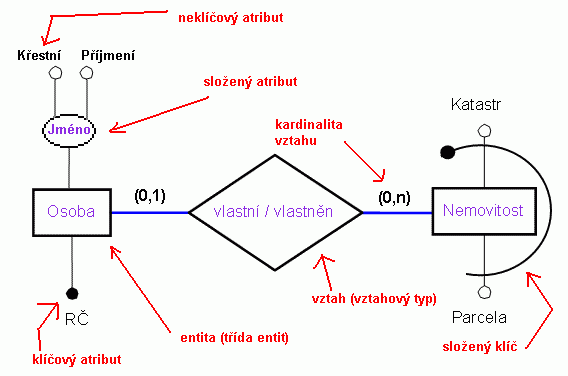
\includegraphics[width=14cm]{informatika/databazy/obrazky/er-schema.png}

(Obrázek je upravený, rozšířený a popsaný příklad ze slidů Dr. T. Skopala k Databázovým systémům)
\end{center}
\end{obecne}

\begin{obecne}{Logické schéma}
\emph{Logické schéma} je datový model organizace nějakého specifického celku pomocí jednoho z databázových modelů -- podle databázových modelů popsaných v předchozí sekci, tj. např. pomocí relačních tabulek, objektových tříd nebo XML. Svojí úrovní abstrakce se nachází mezi konceptuálním a fyzickým schématem.

TODO: to zřejmě nebyl dobrý nápad nacpat datové modely do architektur DB -- vhodnější by to bylo přesunout, je to ale nutné trochu učesat aby seděla terminologie.
\end{obecne}

\begin{obecne}{Fyzické schéma}
\emph{Fyzické datové modely} jsou modely, ktere používají databazové stroje směrem k nižším vrstvám (operačního) systému. V zásadě jde o různé způsoby fyzického uložení dat (tedy schémata organizace souborů) -- sekvenční soubory, B-stromy apod.
\end{obecne}


\subsection{Algoritmy návrhu schémat relací}


\subsubsection*{Normální formy}

\begin{obecne}{Normalizace, anomálie}
Normalizace databází je technika návrhu relačních databázových tabulek, pri které se minimalizují duplicity informací - a zamezuje se tak nekonzistentnosti dat. Stupně normalizace se \uv{popisují} pomocí \emph{normálních forem} - čím vyšší forma, tým vyšší striktnost...

Problémy řešené normalizací:
\begin{pitemize}
	\item \emph{update anomaly} -- př.: tabulka (člověk, adresa, skill); kdyby se nevykonal update správně, může tabulka zůstat v nekonzistentním stavu (např. by se mohly změnit jen některé adresy jednoho člověka)
	\item \emph{insertion anomaly} -- za jistých okolností by se některá fakta nedala zaznamenat, např. v tabulce (fakulta, datum založení, kurz) můžeme zaznamenat jen data pro fakulty, které mají kurzy...
	\item \emph{deletion anomaly} -- za jistých okolností by se mohlo stát, že vymazání některých faktů by způsobilo vymazání dat reprezentujících jiná fakta. V předchozí tabulce bude fakulta vymazána úplně, když se vzdá všech kurzů.
\end{pitemize}

Ideálně by relační databáze měla být navržena tak, aby vylučovala možnost takových anomalií. Normalizace obvykle zahrňuje dekomponování nenormalizované tabulky na dvě nebo více tabulek takových, že po jejich spojení (join) dostaneme všechny původní informace.

Abychom mohli definovat normální formy, potřebujeme znát funkční závislosti jednotlivých atributů entit relační databáze a vědět, které atributy jsou klíčové a které ne.
\end{obecne}

\begin{definiceN}{Funkční závislosti}

\medskip\noindent
Řekneme, že atribut \emph{B} je \textbf{funkčně závislý} na atributu \emph{A}
(značíme $A\rightarrow B$), jestliže pro každou hodnotu atributu \emph{A}
existuje právě jedna hodnota atributu \emph{B}. Rozšířené funkční závislosti se definují pro množinu atributů (pro každou $n$-tici atributů z nějaké množiny existuje právě jedna hodnota závislého(závislých) atributu(atributů)).

Funkční závislosti splňují tzv. \emph{Armstrongova pravidla}, což zahrnuje pro množiny atributů $X,Y,Z$:
\begin{penumerate}
    \item triviální závislost: $X\supseteq Y\ \Rightarrow\ X\to Y$
    \item transitivitu: $X\to Y \wedge Y\to Z\ \Rightarrow\ X\to Z$
    \item kompozici: $X\to Y \wedge X\to Z\ \Rightarrow X\to YZ$
    \item dekompozici: $X\to YZ \ \Rightarrow \ X\to Y \wedge X\to Z$
\end{penumerate}
\end{definiceN}

\begin{definiceN}{Klíč}
\textbf{Nadklíčem}, někdy též \textbf{superklíčem}, schématu $A$ rozumíme každou
podmnožinu množiny $A$, na níž $A$ funkčně závisí. Jinak řečeno nadklíč je množina
atributů, která jednoznačně určuje řádek tabulky.

\textbf{Klíč}, nebo také \textbf{potenciální klíč}(candidate key), schématu $A$
je takový nadklíč schématu $A$, jehož žádná vlastní podmnožina není nadklíčem
$A$. Čili minimální nadklíč.

Každý atribut, který je obsažen alespoň v jednom potenciálním klíči se nazývá
\textbf{klíčový}, ostatní atributy jsou \textbf{neklíčové}.
\end{definiceN}

\begin{definiceN}{Normální formy}
\begin{pitemize}
	\item \emph{První normální forma} \\ -- Tabulka je v první normální formě, jestliže lze do každého pole dosadit pouze jednoduchý datový typ (jsou dále nedělitelné). To zahrnuje i neexistenci více sloupců tabulky se stejným druhem obsahu:
$$
\left.\begin{aligned}
\textrm{(manager, podřízený1, podřízený2, podřízený3)} \\ 
\textrm{(manager, podřízení-vice\_hodnot\_v\_jednom\_sloupci)} \\
\end{aligned}\right\} \rightarrow \textrm{(manager, podřízený)}
$$
	\item \emph{Druhá normální forma} \\ 
-- Existuje klíč a všechna neklíčová pole jsou funkcí celého klíče (a tedy ne jen jeho částí). 
$$\textrm{(custID, name, address, city, state, zip)} \rightarrow
\begin{aligned}&\textrm{(custID, name, address, zip)}\\
&+ \textrm{(zip, city, state)}
\end{aligned}$$
	\item \emph{Třetí normální forma} \\ -- Tabulka je ve třetí normální formě, jestliže každý neklíčový atribut není transitivně závislý na žádném klíči schématu (resp. každý neklíčový atribut je přímo závislý na klíči schématu) neboli je-li ve druhé normální formě a zároveň neexistuje jediná závislost neklíčových sloupců tabulky. 
$$\textrm{(deptID, deptName, managerID, hireDate)} \rightarrow \textrm{(deptID, deptName, managerID)}$$
Atribut \uv{hireDate} je sice funkčně závislý na klíči deptID, ale jen proto, že hireDate závisí na managerID, které závisí na deptID.
	\item \emph{Boyce-Coddova normální forma}\\ -- Pro každou netriviální závislost $X \rightarrow Y$ platí, že $X$ obsahuje klíč schématu $R$ ($X$ je nadklíč).
\end{pitemize}
\end{definiceN}

\subsubsection*{Algoritmy návrhu schémat relací}

Schémata relací by měla být navrhována tak, aby odpovídala předem připravenému konceptuálnímu modelu (např. pomocí ER diagramů) a zároveň pokud možno splňovala co nejpřísnější požadavky na normální formy. Pro modelování relační databáze existují dva přístupy:
\begin{penumerate}
    \item Získání množiny relačních schémat (ručně nebo převodem z např. ER diagramu) a provádění normalizace pro každou tabulku zvlášť
    \item Návrh tzv. univerzálního schématu databáze -- jedna velká tabulka pro celou databázi (vč. platných funkčních závislostí) a normalizace prováděná globálně
\end{penumerate}
První možnost je relativně intuitivní (s ER diagramy) a jednoduchá, ale hrozí riziko přílišného rozdrobení databáze na velký počet malých tabulek (a nadbytečný i vzhledem k požadované normální formě). V druhém způsobu jsou entity jednotlivých relací \uv{vypozorovány} jako efekt funkčních závislostí, což není příliš průhledné a jednoduše proveditelné, ale minimalizuje to šanci na rozdrobení databáze. Oba přístupy lze také zkombinovat -- převést ER model databáze do schémat a některá (nebo až všechna) potom před normalizací sloučit.

\begin{obecne}{Normalizace}
Jediným způsobem, jak u nějakého obecného relačního schématu dosáhnout normální formy (obecně se požaduje většinou 3NF nebo BCNF), je rozdělení na několik podschémat. Dá se to provést ručně nebo algoritmicky a existuje více přístupů podle požadavku na normální formu, \emph{bezztrátovost} (dekompozice relace $R( A, F )$ do $R_1(A_1,F_1)$ a $R_2(A_2,F_2)$ je bezeztrátová, když $A1 \cap A2\to A1$ nebo $A1 \cap A2 \to A2$, tedy opětovným spojením do původní relace nevzniknou další řádky) nebo \emph{pokrytí závislostí} (dekompozice $R(A,F)$ do $R_1(A_1,F_1)$ zachovává pokrytí závislostí, když $F^{+}=F^{+}_1\cup F^{+}_2$ -- nesmí se ztratit závislost ani v rámci dílčího schématu, ani jdoucí napříč schématy).
\end{obecne}

\begin{algoritmusN}{Dekompozice}
Dekompozice je algoritmus, který relační schéma převede do Boyce-Coddovy normální formy. Zaručuje zachování bezeztrátovosti, ale už ne pokrytí závislostí (bez ohledu na algoritmus toto u BCNF někdy není možné). Jeho běh vypadá následovně:
\begin{penumerate}
    \item Vyber nějaké schéma, které není v BCNF.
    \item Vezmi pro něj neklíčovou závislost $X\to Y$ (tak že $X$ není klíč) a dekomponuj podle ní -- vyhoď ze schématu $Y$ a dej $XY$ do zvláštní tabulky.
    \item Opakuj od kroku 1, dokud existuje schéma, které není v BCNF.
\end{penumerate}
\end{algoritmusN}

\begin{algoritmusN}{Syntéza}
Algoritmus syntézy obecně dosahuje třetí normální formy a zachovává pokrytí závislostí (ale ne bezeztrátovost). Pro relační schéma $R$ s množinou funkčních závislostí $F$ vypadá následovně:
\begin{penumerate}
    \item Udělej minimální pokrytí $F$ (vzhledem k tranzitivitě), nazvi ho $G$.
    \item Sluč funkční závislosti z $G$ se stejnou levou stranou a z každé vytvoř jedno schéma. 
    \item Zahoď schémata, která jsou podmnožiny jiných.
\end{penumerate}
Nakonec je možné sloučit schémata s funkčně ekviv. klíči ($K1 \leftrightarrow K2$), ale může to porušit normální formu, které bylo dosaženo! Pro zachování bezeztrátovosti lze do přidat nějaké schéma, obsahující univerzální klíč celého původního (neděleného) schématu.
\end{algoritmusN}

\begin{poznamka}
Pro nalezení minimálního pokrytí atributů se používá pomocný algoritmus, který se chová takto:
\begin{penumerate} 
    \item Dekomponuj všechny funkční závislosti na elementární (na pravé straně je jen jeden sloupec)
    \item Odstraň z nich redundantní atributy (takové z levé strany, které funkčně závisí na jiných z levé strany)
    \item Odstraň redundantní funkční závislosti (tj. takové, které jsou tranzitivním důsledkem jiných -- pravá strana funkčně závisí na levé, i když z množiny funkčních závislostí onu redundantní odstraním)
\end{penumerate}
Pro druhý i třetí krok je potřeba získat \emph{atributový uzávěr} (množina všech atributů i tranzitivně závislých na levé straně) -- to se opakovaně zkouší, jestli díky funkčním závislostem nedostanu z atributů původní množiny nějaké další atributy (dokud nacházím další, přidávám je do množiny a opakuji).
\end{poznamka}

\subsubsection*{Referenční integrita}

\begin{pitemize}
	\item pomáhá udržovat vztahy v relačně propojených databázových tabulkách, zabraňuje vzniku nekonzistentních dat
	\item kontrola přípustných hodnot
	\item kontrola existence položky s daným klíčem v druhé tabulce (podle cizího klíče) 
\end{pitemize}

Chování při porušení integrity:
\begin{pitemize}
	\item ON UPDATE, ON DELETE - podmínka spuštění akce
	\item ON \dots RESTRICT - defaultní řešení (hlášení chyby)
	\item CASCADE - kaskádová aktualizace/smazání (smaže příslušné řádky v odkazované tabulke)
	\item SET NULL - nastavení odkazovaných řádků závislé tabulky na NULL
	\item SET DEFAULT - nastavení pevně určené hodnoty
	\item NO ACTION 
\end{pitemize}

\subsection{Transakční zpracování, vlastnosti transakcí, uzamykací protokoly, zablokování}

\begin{definiceN}{Transakce}
\emph{Transakce} je jistá posloupnost nebo specifikace posloupnosti akcí práce s databází, jako
jsou čtení, zápis nebo výpočet, se kterou se zachází jako s jedním celkem.
\end{definiceN}

Hlavním smyslem používání transakcí, tj. \emph{transakčního zpracování}, je
udržení databáze v konzistentním stavu. Jestliže na sobě některé operace závisí,
sdružíme je do jedné transakce a tím zabezpečíme, že budou vykonány buď
všechny, nebo žádná. Databáze tak před i po vykonání transakce bude v
konzistentním stavu. Aby se uživateli transakce jevila jako jedna atomická
operace, je nutné zavést příkazy COMMIT a ROLLBACK. První z nich signalizuje
databázi úspěšnost provedení transakce, tj. veškeré změny v databázi se stanou
trvalými a jsou zviditelněny pro ostatní transakce, druhý příkaz signalizuje
opak, tj. databáze musí být uvedena do původního stavu.

Tyto příkazy většinou není nutné volat explicitně, např. příkaz COMMIT je vyvolán po
normálním ukončení programu realizujícího transakci. Příkaz ROLLBACK pro svou
funkci vyžaduje použití tzv. \emph{žurnálu} (logu) na nějakém stabilním
paměťovém médiu. Žurnál obsahuje historii všech změn databáze v jisté časové
periodě.

Jednoduchá transakce vypadá většinou takto:
\begin{penumerate}
  \item Začátek transakce,
  \item provedení několika dotazů -- čtení a zápisů (žádné změny v databázi nejsou zatím vidět pro
  okolní svět),
  \item Potvrzení (příkaz COMMIT) transakce (pokud se transakce povedla, změny
  v databázi se stanou viditelné).
\end{penumerate}
Pokud nějaký z provedených dotazů selže, systém by měl celou transakci zrušit a
vrátit databázi do stavu v jakém byla před zahájením transakce (operace ROLLBACK).

Transakční zpracování je také ochrana databáze před hardwarovými nebo
softwarovými chybami, které mohou zanechat databázi po částečném zpracování
transakce v nekonzistentním stavu. Pokud počítač selže uprostřed provádění
některé transakce, transakční zpracování zaručí, že všechny operace z
nepotvrzených (\uv{uncommitted}) transakcí budou zrušeny. 

\subsubsection*{Vlastnosti transakcí}

Podívejme se nyní na vlastnosti požadované po transakcích. Obvykle se používá
zkratka prvních písmen anglických názvů vlastností \textbf{ACID}~-- atomicity,
consistency, isolation (independence), durability. 
\begin{description}
  \item[atomicita] -- transakce se tváří jako jeden celek, musí buď proběhnout
  celá, nebo vůbec ne.
  \item[konzistence] -- transakce transformuje databázi z jednoho konzistentního
  stavu do jiného konzistentního stavu.
  \item[nezávislost] -- transakce jsou nezávislé, tj. dílčí efekty transakce
  nejsou viditelné jiným transakcím.
  \item[trvanlivost] -- efekty úspěšně ukončené (potvrzené,\uv{commited})
  transakce jsou nevratně uloženy do databáze a nemohou být zrušeny.
\end{description}

Transakce mohou být v uživatelských programech prováděny paralelně (spíše
zdánlivě paralelně, stejně jako je paralelismus multitaskingu na jednoprocesorových
strojích jen zdánlivý, zajistí to ale možnost paralelizace \uv{nedatabázových} 
akcí a pomalé transakce nebrzdí rychlé). Je
zřejmé, že posloupnost transakcí může být zpracována paralelně různým způsobem.
Každá transakce se skládá z několika akcí. Stanovené pořadí provádění akcí
více transakcí v čase nazveme \textbf{rozvrhem}.

Rozvrh, který splňuje následující podmínky, budeme nazývat \textbf{legální}:
\begin{pitemize}
  \item Objekt je nutné mít uzamknutý, pokud k němu chce transakce přistupovat.
  \item Transakce se nebude pokoušet uzamknout objekt již uzamknutý jinou
  transakcí (nebo musí počkat, než bude objekt odemknut).
\end{pitemize}

Důležitými pojmy pro paralelní zpracování jsou sériovost či uspořádatelnost.
\textbf{Sériové rozvrhy} zachovávají operace každé transakce pohromadě (a 
provádí se jen jedna transakce najednou). Pro $n$
transakcí tedy existuje $n!$ různých sériových rozvrhů. Pro získání korektního
výsledku však můžeme použít i rozvrhu, kde jsou operace různých transakcí
navzájem prokládány.
Přirozeným požadavkem na korektnost je, aby efekt paralelního zpracování
transakcí byl týž, jako kdyby transakce byly provedeny v nějakém sériovém rozvrhu.
Předpokládáme-li totiž, že každá transakce je korektní program, měl by vést
výsledek sériového zpracování ke konzistentnímu stavu. O systému zpracování
transakcí, který zaručuje dosažení konzistentního stavu nebo stejného stavu
jako sériové rozvrhy, se říká, že zaručuje \textbf{uspořádatelnost}.

Mohou se vyskytnout problémy, které uspořádatelnosti zamezují. Ty nazýváme \emph{konflikty}. Plynou z pořadí dvojic akcí různých transakcí na stejném objektu. Existují tři typy konfliktních situací:
\begin{penumerate}
    \item WRITE-WRITE -- přepsání nepotvrzených dat
    \item READ-WRITE -- neopakovatelné čtení
    \item WRITE-READ -- čtení nepotvrzených (\uv{uncommitted}) dat
\end{penumerate}

Řekneme, že rozvrh je \emph{konfliktově uspořádatelný}, je-li konfliktově ekvivalentní nějakému sériovému rozvrhu (tedy jsou v něm stejné, tj. žádné konflikty). Test na konfliktovou uspořádatelnost se dá provést jako test acykličnosti grafu, ve kterém konfliktní situace představují hrany a transakce vrcholy. Konfliktová uspořádatelnost je slabší podmínka než uspořádatelnost -- nezohledňuje ROLLBACK (\emph{zotavitelnost} -- zachování konzistence, i když kterákoliv transakce selže) a dynamickou povahu databáze (vkládání a mazání objektů). Zotavitelnosti se dá dosáhnout tak, že každá transakce $T$ je potvrzena až poté, co jsou potvrzeny všechny ostatní transakce, které změnily data čtená v $T$. Pokud v zotavitelném rozvrhu dochází ke čtení změn pouze potvrzených transakcí, nemůže dojít ani k jejich \emph{kaskádovému rušení}.

Při zpracování (i uspořádatelného) rozvrhu může dojít k situaci \emph{uváznutí} -- \emph{deadlocku}. To nastane tehdy, pokud jedna transakce $T_1$ čeká na zámek na objekt, který má přidělený $T_2$ a naopak. Situaci lze zobecnit i na více transakcí. Uváznutí lze buď přímo zamezit charakterem rozvrhu, nebo detekovat (hledáním cyklu v grafu čekajících transakcí, tzv. \uv{waits-for} grafu) a jednu z transakcí \uv{zabít} a spustit znova.

\medskip
K zajištění uspořádatelnosti a zotavitelnosti a zabezpečení proti kaskádovým rollbackům a deadlocku se používají různá schémata (požadavky na rozvrhy). Jedním z nich jsou uzamykací protokoly.

\subsubsection*{Uzamykací protokoly}

Vytváření rozvrhů a testování jejich uspořádatelnosti není pro praxi zřejmě ten
nejvhodnější způsob. Pokud ale budeme transakce konstruovat podle určitých
pravidel, tak za určitých předpokladů bude každý jejich rozvrh uspořádatelný.
Soustavě takových pravidel se říká \textbf{protokol}.

Nejznámější protokoly jsou založeny na dynamickém zamykání a odemykání objektů v
databázi. Zamykání (operace LOCK) je akce, kterou vyvolá transakce na objektu,
aby ho chránila před přístupem ostatních transakcí.

\begin{definiceN}{Dobře formovaná transakce}
Transakci nazveme \textbf{dobře formovanou} pokud podporuje přirozené požadavky
na transakce:
\begin{penumerate}
  \item transakce zamyká objekt, chce-li k němu přistupovat,
  \item transakce nezamyká objekt, který již je touto transakcí uzamčený,
  \item transakce neodmyká objekt, který není touto transakcí zamčený,
  \item po ukončení transakce jsou všechny objekty uzamčené touto transakcí
  odemčeny.
\end{penumerate}
\end{definiceN}

\paragraph{Dvoufázový protokol (2PL)} -- Dvoufázová transakce v první fázi
zamyká vše co je potřeba a od prvního odemknutí (druhá fáze) již jen odemyká co
měla zamčeno (již žádná operace LOCK). Tedy transakce musí mít všechny objekty
uzamčeny předtím, než nějaký objekt odemkne. Dá se dokázat, že pokud jsou
všechny transakce v dané množině transakcí dobře formované a dvoufázové, pak
každý jejich legální rozvrh je uspořádatelný.

Dvoufázový protokol zajišťuje uspořádatelnost, ale ne zotavitelnost ani
bezpečnost proti kaskádovému rušení transakcí nebo uváznutí.

\paragraph{Striktní dvoufázový protokol (S2PL)} -- Problémy 2PL jsou nezotavitelnost
a kaskádové rušení transakcí. Tyto nedostatky lze odstranit pomocí striktních
dvoufázových protokolů, které uvolňují zámky až po skončení transakce (COMMIT).
Zřejmá nevýhoda je omezení paralelismu. 2PL navíc stále nevylučuje možnost deadlocku.

\paragraph{Konzervativní dvoufázový protokol (C2PL)} -- Rozdíl oproti 2PL je
ten, že transakce žádá o všechny své zámky, ještě než se začne
vykonávat. To sice vede občas k zbytečnému zamykání (nevíme co přesně budeme
potřebovat, tak radši zamkneme víc), ale stačí to již k prevenci uváznutí
(deadlocku).

\subsubsection*{\uv{Vylepšení} zamykacích protokolů}

\paragraph{Sdílené a výlučné zámky} -- Nevýhodou 2PL je, že objekt může mít
uzamčený pouze jedna transakce. Abychom uzamykání provedli precizněji, je dobré
vzít na vědomí rozdíl mezi operacemi READ a WRITE. \emph{Výlučný zámek}
(W\_LOCK) může být aplikován na objekty jak pro operaci READ tak pro WRITE,
\emph{sdílený zámek} (R\_LOCK) uzamyká objekt, který chceme pouze číst. Jeden
objekt potom může být uzamčen sdíleným zámkem více transakcí a zvyšuje se tak
možnost paralelního zpracování. Budeme-li s těmito zámky zacházet stejně jako u
2PL, opět máme zaručenou uspořádatelnost rozvrhu, ovšem nikoliv absenci uváznutí.


\paragraph{Strukturované uzamykání (multiple granularity)} -- Objekty jsou v
tomto případě chápány hierarchicky dle relace \emph{obsahuje}. Například
databáze obsahuje soubory, které obsahují stránky a ty zase obsahují jednotlivé
záznamy. Na tuto hierarchii se můžeme dívat jako na strom, ve kterém každý
vrchol obsahuje své potomky. Když transakce zamyká objekt (vrchol) zamyká také
všechny jeho potomky. Protokol se tak snaží minimalizovat počet zámků, tím
snížit režii a zvýšit možnosti paralelního zpracování.


\subsubsection*{Alternativní protokoly}

\paragraph{Časová razítka} -- Další z protokolů zaručující uspořádatelnost je
využití časových razítek. Na začátku dostane transakce $T$ \emph{časové
razítko}~-- $TS(T)$ (časová razítka jsou unikátní a v čase rostou), abychom věděli
pořadí, ve kterém by měli být transakce vykonány. Každý objekt v databázi má
\emph{čtecí razítko}~-- $RTS(O)$ (read timestamp), které je aktualizováno, když je
objekt čten, a \emph{zapisovací razítko}~-- $WTS(O)$ (write timestamp), které je
aktualizováno, když nějaká transakce objekt mění.

Pokud chce transakce $T$ číst objekt $O$ mohou nastat dva případy:
\begin{pitemize}

  \item $TS(T) < WTS(O)$, tzn. někdo změnil objekt $O$ potom co byla spuštěna
  transakce $T$. V tomto případě musí být transakce zrušena a spouštěna znovu (a
  tedy s jiným časovým razítkem).

  \item $TS(T) > WTS(O)$, tzn. je bezpečné objekt číst. V tomto případě $T$
  přečte $O$ a $RTS(O)$ je nastaveno na $\max\{TS(T),\ RTS(O)\}$.

\end{pitemize}

Pokud chce transakce $T$ zapisovat do objektu $O$ rozlišujeme případy tři:
\begin{pitemize}

  \item $TS(T) < RTS(O)$, tzn. někdo četl $O$ poté co byla spuštěna $T$ a
  předpokládáme, že si pořídil lokální kopii. Nemůžeme tedy $O$ změnit, protože
  by lokální kopie přestala být platná a tedy je nutné $T$ zrušit a spustit
  znova.

  \item $TS(T) < WTS(O)$, tzn. někdo změnil $O$ po startu $T$. V tomto případě
  přeskočíme write operaci a pokračujeme dále normálně. $T$ nemusí být
  restartována.

  \item V ostatních případech $T$ změní $O$ a $WTS(O)$ je nastaveno na $TS(T)$.
\end{pitemize}

\paragraph{Optimistické protokoly} -- V situaci kdy se většina transakcí
neovlivňuje, je režie výše uvedených protokolů zbytečně velká a můžeme použít
takzvaný optimistický protokol. V protokolu můžeme rozlišit tři fáze.
\begin{penumerate}

  \item \textbf{Fáze čtení:} Čtou se objekty z databáze do lokální paměti a jsou
  na nich prováděny potřebné změny.

  \item \textbf{Fáze kontroly:} Po dokončení všech změn v lokální paměti je
  vyvolán pokus o zapsání výsledků do databáze. Algoritmus zkontroluje, zda
  nehrozí potenciální kolize s již potvrzenými transakcemi, nebo s některými
  právě probíhajícími. Pokud konflikt existuje, je třeba spustit algoritmus pro
  řešení kolizí, který se je snaží vyřešit. Pokud se mu to nepodaří, je využita
  poslední možnost a tou je zrušení a restartování transakce.

  \item \textbf{Fáze zápisu:} Pokud nehrozí žádné konflikty, jsou data z lokální
  paměti zapsány do databáze a transakce potvrzena.

\end{penumerate}



\subsection{ER-diagramy, metody návrhu IS}

ER-diagramy jsou de-facto standard pro konceptuální datové modelování. Jsou vhodné hlavně pro \uv{plochá} neformátovaná data, tj. hlavně pro relační, objektově-relační nebo objektové databáze. Nejsou vhodné pro multimediální nebo hierarchická data (jako např. XML). E-R v názvu znamená \emph{entity-relationship} modelování, tedy modelování s pomocí (tříd) entit a jejich vztahů. ER model databáze definuje její konceptuální schéma. Jde vlastně o obdobu UML schémat v objektovém programování.

\begin{obecne}{Entitní typ}
\emph{Entitní typ} (v diagramu se značí hranatým rámečkem) reprezentuje nějakou třídu entit (např. \uv{Zaměstnanec}). Každý entitní typ má nějaké \emph{atributy} (např. \uv{jméno}), z nichž některé mohou být \emph{identifikátory}, tj. takové, které jednoznačně určují instanci entity. Pokud nemá žádné identifikátory explicitně označené, jsou jimi všechny atributy dohromaty (tzv. složený identifikátor). Identifikátory mohou být i víceatributové. 

Atributy entitních typů mohou být \emph{jednoduché} nebo \emph{složené}, \emph{povinné} či \emph{nepovinné}, případně \emph{jednohodnotové} a \emph{vícehodnotové}. Jejich zobrazení ukazuje následující obrázek:

\begin{center}
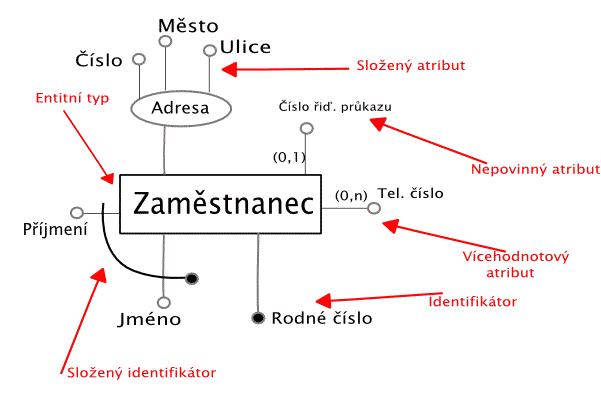
\includegraphics[width=14cm]{informatika/databazy/obrazky/er1.png}

(Entitní typ se všemožnými druhy atributů)
\end{center}
\end{obecne}

\begin{obecne}{Vztahový typ}
\emph{Vztahový typ} (v diagramu značený kosočtvercem) popisuje vztahy mezi jednotlivými entitami -- s těmi entitami, se kterými je v nějakém vztahu, je spojen čarou. Vztah může mít danou i \emph{kardinalitu} (kolik entit z každé strany do vztahu vstupuje), která může být typu $1:1$, $1:n$, $m:n$ a je značená vedle čáry spojující vztahový typ s entitou. Entity ve vztahu mohou mít navíc \emph{povinné či nepovinné členství} (vstupovat do něj vždy nebo jen někdy).

Vztahy mohou být buď binární nebo obecně $n$-ární, ale více než ternární vztahy se většinou neobjevují. Vztahy mohou být i rekurzivní, tj. do vztahů vstupují entity stejného typu. Instance vztahového typu je jednoznačně určena identifikátory instancí entit ve vztahu. Některé entitní typy mohou být spoluidentifikovány (nebo přímo identifikovány) vztahem -- pak se nazývají \emph{slabé entitní typy}.

\begin{center}
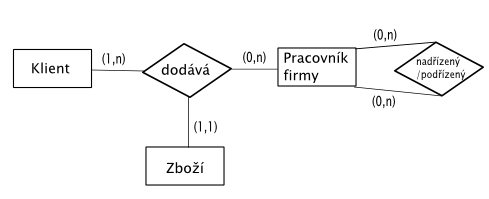
\includegraphics[width=12cm]{informatika/databazy/obrazky/er2.png}

(Vztahové typy)
\end{center}
Obrázek ukazuje ternární vztah s různými kardinalitami -- klientovi někdo dodává zboží jednou až $n$-krát, pracovník dodává nula až $n$-krát zboží (tj. jde o nepovinné členství ve vztahu, můžou existovat pracovníci, kteří nic nedodávají) a zboží je vždy někomu dodáváno právě jednou. Na zaměstnancích je zároveň ukázán rekurzivní binární vztah.


\begin{center}
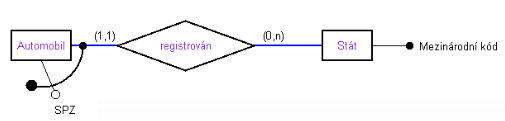
\includegraphics[width=10cm]{informatika/databazy/obrazky/er3.png}

(Slabý entitní typ. Zdroj: slidy Dr. T. Skopala k Databázovým systémům)
\end{center}
Tento obrázek ukazuje, jak vypadá slabý entitní typ -- automobil je identifikován svojí SPZ a zároveň státem, ve kterém je registrován.
\end{obecne}


\begin{obecne}{ISA hierarchie}
ISA hierarchie je rozšíření ER diagramů o \uv{dědičnost} entit -- tj. rozdělení entitních typů na subtypy (a přidání dalších vztahů nebo atributů pro subtypy). V ISA hierarchii se povoluje pouze jednonásobná dědičnost, navíc potomci nějakého entitního typu musí být jednoznačně identifikováni předkem (tj. všechny entity v hierarchii sdílí identifikátor).

\begin{center}
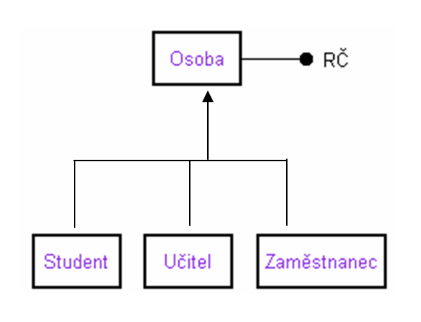
\includegraphics[width=6cm]{informatika/databazy/obrazky/er4.png}

(ISA hierarchie. Zdroj: slidy Dr. T. Skopala k Databázovým systémům)
\end{center}
\end{obecne}

\begin{obecne}{Úpravy ER diagramů}
V ER diagramu je možné provádět víceméně \uv{ekvivalentní} úpravy (výsledný diagram reprezentuje stejný koncept databáze), např. pro odstranění vztahů s kardinalitou $m:n$ (převod na dva vztahy kardinalitami $1:n$ a \emph{průnikový entitní typ}, který je vztahy určený, takže je slabý). Dalším důvodem úprav může být zbavení se ISA hierarchie. To se dá provést více způsoby, přičemž žádný z nich nefunguje úplně obecně:
\begin{pitemize}
    \item agregace atributů a vztahů potomka do předka a úprava kardinalit (převod na nepovinné atributy a nepovinné členství ve vztahu)
    \item odstranění předka a duplikace všech jeho atributů a vztahů v potomcích
    \item nahrazení ISA vztahu klasickým vztahem (z potomků vzniknou slabé entitní typy)
\end{pitemize}
Jiná úprava je odstranění vícehodnotového atributu -- převede se na vztah s kardinalitou $1:n$ a slabý entitní typ.
\end{obecne}

\begin{obecne}{Korektní ER schéma}
V \emph{korektním} ER schématu všechny entity a vztahy splňují:
\begin{pitemize}
    \item Žádný entitní typ nemá více než jednoho ISA předka.
    \item ISA vztahy netvoří orientovaný cyklus.
    \item Identifikační vztahy netvoří orientovaný cyklus.
    \item Potomek v ISA hierarchii není identifikačně závislý na žádném entitním typu (je již identifikován předkem).
    \item Jména entitních a vztahových typů jsou jednoznačná.
\end{pitemize}
\end{obecne}


TODO: Co je ksakru \uv{ metody návrhů IS}?

\subsection{SQL}

Zdroje: slidy z přednášek Databázové systémy a Databázové aplikace Dr. T. Skopala a Dr. M. Kopeckého.

\subsubsection*{Standardy SQL}

SQL (\emph{Structured query language}) je standardní jazyk pro přístup k relačním databázím (a dotazování nad nimi). Je zároveň jazykem pro definici dat (definition data language), vytváření a modifikace schémat (tabulek), manipulaci s daty (data manipulation language), vkládání, aktualizace, mazání dat, řízení transakcí, definici integritních omezení aj. Jeho syntaxe odráží snahu o co nejpřirozenější formulace požadavků -- je podobná anglickým \uv{větám}.

SQL je standard podle norem ANSI/ISO a existuje v několika (zpětně kompatibilních) verzích (označovaných podle roku uvedení):
\begin{description}
    \item[SQL 86] -- první \uv{nástřel}, průnik implementací SQL firmy IBM
    \item[SQL 89] -– malá revize motivovaná komerční sférou, mnoho detailů ponecháno implementaci
    \item[SQL 92] –- mnohem silnější a obsáhlejší jazyk. Zahrnuje už
    \begin{pitemize}
	\item modifikace schémat, tabulky s metadaty, 
	\item vnější spojení, množinové operace
	\item kaskádové mazání/aktualizace podle cizích klíčů, transakce
	\item kurzory, výjimky
    \end{pitemize}
    Standard existuje ve čtyřech verzích: Entry, Transitional, Intermediate a Full.
    \item[SQL 1999] -– přináší mnoho nových vlastností, např. 
    \begin{pitemize}	
	\item objektově-relační rozšíření
	\item nové datové typy -- reference, pole, full-text
	\item podpora pro externí datové soubory, multimédia
	\item triggery, role, programovací jazyk, regulární výrazy, rekurzivní dotazy ...
    \end{pitemize}
    \item[SQL 2003] -– další rozšíření, např. XML management
\end{description}

Komerční systémy implementují SQL podle různých norem, někdy jenom SQL-92 Entry, dnes nejčastěji SQL-99, ale nikdy úplně striktně. Některé věci chybí a naopak mají všechny spoustu nepřenositelných rozšíření -- např. specifická rozšíření pro procedurální, transakční a další funkcionalitu (T-SQL (Microsoft SQL Server), PL-SQL (Oracle) ). S novými verzemi se kompatibilita zlepšuje, často je možné používat obojí syntax. Přenos aplikace za běhu na jinou platformu je ale stále velice náročný -- a to tím náročnější, čím víc věcí mimo SQL-92 Entry obsahuje. Pro otestování, zda je špatně syntax SQL, nebo zda jen daná databázová platforma nepodporuje některý prvek, slouží SQL validátory (které testují SQL podle norem).


\subsubsection*{Dotazy v SQL}

Hlavním nástrojem dotazů v SQL je příkaz \texttt{SELECT}. Sdílí prvky relačního kalkulu i relační algebry -- obsahuje práci se sloupci, kvantifikátory a agregační funkce z relačního kalkulu a další operace -- projekce, selekce, spojení, množinové operace -- z relační algebry. Na rozdíl od striktní formulace relačního modelu databáze povoluje duplikátní řádky a NULLové hodnoty atributů.

Netříděný dotaz v SQL sestává z:
\begin{pitemize}
    \item příkazu(ů) \texttt{SELECT} (hlavní logika dotazování), to obsahuje vždy
    \item může obsahovat i množinové operace nad výsledky příkazů \texttt{SELECT} -- \texttt{UNION}, \texttt{INTERSECTION} ...
\end{pitemize}
Výsledky nemají definované uspořádání (resp. jejich pořadí je určeno implementací vyhodnocení dotazu).

Příkaz \texttt{SELECT} vypadá následovně (tato verze už zahrnuje i třídění výsledků):
\begin{verbatim}
SELECT [DISTINCT]
 výraz1 [[AS] c_alias1] [, ...]
FROM
 zdroj1 [[AS] t_alias1] [, ...]
[WHERE podmínka_ř]
[GROUP BY výraz_g1 [, …]
[HAVING podmínka_s]]
[ORDER BY výraz_o1 [, …] ASC/DESC]
\end{verbatim}
Kde
\begin{pitemize}
    \item výrazy mohou být sloupce, sloupce s agregačními funkcemi, výsledky dalších funkcí ...

\noindent \texttt{ výraz = <název sloupce>, <konstanta>, \\
 (DISTINCT) COUNT(~<název sloupce>~),\\
{}[DISTINCT] [~SUM~|~AVG~](~<výraz>~),\\
{}[~MIN~|~MAX~](~<výraz>~)}\\
a navíc lze použít operátory $+,-,*,/$.

    \item zdroje jsou tabulky nebo vnořené selecty
    \item výrazy i zdroje být přejmenovány pomocí \texttt{AS}, např. pro odkazování uvnitř dotazu nebo jména na výstupu (od SQL-92)
    \item podmínka je logická podmínka (spojovaná logickými spojkami \texttt{AND, OR}) na hodnoty dat ve zdrojích:

\texttt{podmínka = <výraz> BETWEEN <x> AND <y>, <výraz> LIKE "\%\_ ... ",\\
<výraz> IS [NOT] NULL,\\
<výraz> > = <> <= < > [<výraz>/ ALL / ANY <dotaz>],\\
<výraz> NOT IN [<seznam hodnot> / <dotaz>], EXIST ( <dotaz> )}

    \item \texttt{GROUP BY} znamená agregaci podle unikátních hodnot jmenovaných sloupců (v ostatních sloupcích vznikají množiny hodnot, které se spolu s oněmi unikátnímí vyskytují na stejných řádkách
    \item \texttt{HAVING} označuje podmínku na agregaci
    \item \texttt{ORDER BY} definuje, podle hodnot ve kterých sloupcích nebo podle kterých jiných výrazů nad nimi provedených se má výsledek setřídit (\texttt{ASC} požaduje vzestupné setřídění, \texttt{DESC} sestupné).
\end{pitemize}

SQL nemá příkaz na omezení rozsahu na některé řádky (jako např. \uv{potřebuji jen 50.-100. řádek výpisu}), a to lze řešit buď složitě standardně (počítání kolik hodnot je menších než vybraná, navíc náročné na hardware) nebo pomocí některého nepřenositelného rozšíření.

\medskip\noindent
Pořadí vyhodnocování jednoho příkazu \texttt{SELECT} (nebereme v úvahu optimalizace):
\begin{penumerate}
    \item Nejprve se zkombinují data ze všech zdrojů (tabulek, pohledů, poddotazů). Pokud jsou odděleny čárkami, provede se kartézský součin (to samé co \texttt{CROSS JOIN}), v SQL-92 a vyšším i složitější spojení -- \texttt{JOIN ON} (vnitřní spojení podle podmínky), \texttt{NATURAL JOIN} (\uv{přirozené} spojení podle stejných hodnot stejně pojmenovaných sloupců), \texttt{OUTER JOIN} (\uv{vnější} spojení, do kterého jsou zahrnuty i záznamy, pro které v jednom ze zdrojů není nalezeno nic, co by odpovídalo podmínce, doplněnné NULLovými hodnotami) atd.
    \item Vyřadí se vzniklé řádky, které nevyhovují podmínce (\texttt{WHERE})
    \item Zbylé řádky se seskupí do skupin se stejnými hodnotami uvedených výrazů (\texttt{GROUP BY}), každá skupina obsahuje atomické sloupce s hodnotami uvedených výrazů a množinové sloupce se skupinami ostatních hodnot sloupců.
    \item Vyřadí se skupiny, nevyhovující podmínce (\texttt{HAVING})
    \item Výsledky se setřídí podle požadavků
    \item Vygeneruje se výstup s požadovanými hodnotami
    \item V případě \texttt{DISTINCT} se vyřadí duplicitní řádky
\end{penumerate}


\begin{poznamka}
\begin{pitemize}
    \item Klauzule \texttt{GROUP BY} setřídí před vytvořením skupin všechny řádky dle výrazů v klauzuli. Proto by se měl seskupovat co nejmenší možný počet řádek. Pokud je možné řádky odfiltrovat pomocí WHERE, je výsledek efektivnější, než následné odstraňování celých skupin.
    \item  Klauzule \texttt{DISTINCT} třídí výsledné záznamy (před operací ORDER BY), aby našla duplicitní záznamy. Pokud to jde, je vhodné se bez ní obejít.
    \item Klauzule \texttt{ORDER BY} by měla být použita jen v nutných případech. Není příliš vhodné ji používat v definicích pohledů, nad kterými se dále dělají další dotazy.
\end{pitemize}
\end{poznamka}


\subsubsection*{Definice a manipulace s daty, ostatní příkazy}

Standard SQL podporuje několik druhů datových typů:
\begin{pitemize}
    \item textové v národní a globální (UTF) znakové sadě (několika druhů -- proměnné a pevné délky): \texttt{CHARACTER(n)}, \texttt{NCHAR(n)},
    \texttt{CHAR VARYING(n)}
    \item číselné typy -- \texttt{ NUMERIC(p[,s]), INTEGER, INT, SMALLINT,\\  FLOAT(presnost), REAL, DOUBLE PRECISION}
    \item datumové typy -- \texttt{DATE, TIME, TIMESTAMP, TIMESTAMP(presnost\_sekund) WITH TIMEZONE}
\end{pitemize}
Databázové servery ne vždy podporují všechny uvedené typy. Nemusí je podporovat nativně, někdy si pouze \uv{přeloží} název typu na podobný nativně podporovaný typ.

\medskip
\begin{obecne}{Příkaz \texttt{CREATE TABLE}}
Tento příkaz slouží k vytvoření nové tabulky. Je nutné definovat její název, atributy a jejich domény (datové typy); dále je možné definovat integritní omezení (klíče, cizí klíče, odkazy, podmínky). Příkaz vypadá následovně:
\begin{center}
\texttt{CREATE TABLE <název> <def. sloupce/i.o. tabulky, ...> }
\end{center}
A uvnitř potom
\begin{verbatim}
def. sloupce = <název> <dat.typ> 
    [DEFAULT NULL|<hodnota>] [<i.o.sloupce>] 
dat.typ = [VARCHAR(n) | BIT(n) | INTEGER | FLOAT | DECIMAL ...] 
i.o.sloupce = [CONSTRAINT <jméno>] [NOT NULL / UNIQUE / PRIMARY KEY], 
    REFERERENCES <tabulka>(<sloupec>) <akce>, CHECK <podmínka> 
akce = [ON UPDATE / ON DELETE] 
    [CASCADE / SET NULL / SET DEFAULT / NO ACTION(hlášení chyby) ] 
i.o.tabulky = UNIQUE, PRIMARY KEY <sloupec, ... >, 
    FOREIGN KEY <sloupec, ... >, 
    REFERENCES <tabulka>(<sloupec, ... >), 
    CHECK( <podmínka> )
\end{verbatim}
\end{obecne}

\medskip
\begin{obecne}{Příkazy pro manipulaci se schématem}
\begin{pitemize}
    \item Úprava tabulky:
\begin{verbatim}
ALTER TABLE <název> ADD {COLUMN} <def.sloupce>, ADD <i.o.tabulky>, 
    ALTER COLUMN <sloupec> [ SET / DROP ], DROP COLUMN <sloupec>, 
    DROP CONSTRAINT <jméno i.o.> 
\end{verbatim}
    \item Smazání tabulky (není to samé jako vymazání všech dat z tabulky!):
\begin{verbatim}
DROP TABLE <tabulka> 
\end{verbatim}
    \item Vytvoření \uv{pohledu} -- navenek se chová jako tabulka, ale vnitřně se při každém dotazu provede vnořený dotaz (který definicí pohledu zapisuji):
\begin{verbatim}
CREATE VIEW <název "tabulky"> ( <sloupec, ... > ) 
    AS <dotaz> {WITH [ LOCAL / CASCADED ] CHECK OPTION }
\end{verbatim}
    Některé databázové platformy umožňují do takto vytvořených pohledů i zapisovat.
\end{pitemize}
\end{obecne}

\medskip
\begin{obecne}{Příkazy pro manipulaci s daty}
\begin{pitemize}
    \item Vložení nových dat do tabulky
\begin{verbatim}
INSERT INTO <tabulka> ( <sloupec, ... > ) 
    [VALUES ( <výraz, ... > ) / (<dotaz>) ] 
\end{verbatim}
    \item Úprava dat (na řádcích které vyhovují podmínce se nastaví zadané hodnoty vybraným sloupcům):
\begin{verbatim}
UPDATE <tabulka> SET 
    ( <sloupec> = [ NULL / <výraz> / <dotaz> ] , ... ) 
    WHERE (<podmínka>) 
\end{verbatim}
    \item Smazání řádků vyhovujících podmínce z tabulky:
\begin{verbatim}
DELETE FROM <tabulka> ( WHERE <podmínka> ) 
\end{verbatim}
\end{pitemize}
\end{obecne}

TODO: doplnit ?

\subsection{Indexy, triggery, uložené procedury, uživatelé}

TODO: pořádná definice indexu

\begin{obecne}{Index}
Index je obvykle definován výběrem tabulky a jejího konkrétního sloupce (nebo sloupců), nad kterými si designér databáze přeje dotazování urychlit; dále pak technickým určením typu. Chování a způsoby uložení indexů se mohou významně lišit podle použité databázové technologie.
Výjimku mohou tvořit například full-textové indexy, které jsou v některých případech (nerelační databáze typu Lotus Notes) definovány nad celou databází, nikoliv nad konkrétní tabulkou. 
\end{obecne}

\begin{obecne}{Použití indexu}
Na první pohled by se mohlo zdát, že čím víc indexů, tím lepší chování databáze a že po vytvoření indexů pro všechny sloupce všech tabulkách dosáhneme maximálního zrychlení. Tento přístup naráží bohužel na dva zásadní problémy: 
\begin{penumerate}
    \item Každý index zabírá v paměti vyhrazené pro databázi nezanedbatelné množství místa (vzhledem k paměti vyhrazené pro tabulku). Při existenci mnoha indexů se může stát, že paměť zabraná pro jejich chod je skoro stejně velká, jako paměť zabraná jejími daty - zvláště u rozsáhlých tabulek (typu faktových tabulek v datovém skladu) může něco takového být nepřijatelné. 
    \item Každý index zpomaluje operace, které mění obsah indexovaných sloupců (například SQL příkazy UPDATE, INSERT). To je dáno tím, že databáze se v případě takové operace nad indexovaným sloupcem musí postarat nejen o změny v datech tabulky, ale i o změny v datech indexu. 
\end{penumerate}
\end{obecne}

\begin{obecne}{Typy indexů}
Indexy mohou mít svůj typ, který blíže určuje, jakým způsobem má být přistupování k datům tabulky optimalizováno. Označení se různí, ale nejčastěji je to:
\begin{pitemize}
    \item PRIMARY - Tento typ se v každé tabulce může vyskytovat nejvýše jednou. Definuje sloupec tabulky, který svou hodnotou jednoznačně identifikuje záznam. Ve většině případů se dodržuje konvence takový sloupec nazvat ID a jeho datový typ stanovit jako celé číslo (není-li potřeba jinak). Databázový server by měl být schopen nedopustit, aby byla do sloupce, k němuž se tento typ indexu vztahuje, byla vložena hodnota, která již v tabulce existuje (většinou takový pokus končí chybovou hláškou). 
    \item UNIQUE - Tento typ je podobný PRIMARY co do jednoznačnosti záznamu v tabulce (jak naznačuje i jeho název) a dopadu, který to na práci s databází má; ale může se vyskytovat u více sloupců tabulky. Podle účelu, ke kterému má tabulka sloužit, se občas definují indexy složené z více sloupců - potom opět nelze vložit záznam, který by již v této kombinaci někde v tabulce existoval. 
    \item INDEX - Definicí indexu tohoto typu je v tabulce zajištěna optimalizace vyhledávání podle sloupce, ke kterému se daný index váže. Většinou si databázový server vytvoří a nadále udržuje vnitřní seznam odkazů na řádky tabulky, seřazený podle hodnot sloupce, k němuž se váže. Udržování takto seřazené posloupnosti urychluje vyhledávání (je možno použít některé interpolační numerické metody), řazení i jiné zásahy do tabulky, které jsou omezeny podmínkou na dotyčné záznamy. 
    \item FULL-TEXT - Vytvořením tohoto indexu se databázový server bude snažit optimalizovat full-textové vyhledávání v daném sloupci u dané tabulky.
\end{pitemize}
\end{obecne}

\begin{obecne}{Triggery}
  Databázový trigger je programový kód, který je automaticky vykonán jako
  reakce na nějakou událost v určité databázové tabulce. Triggery mohou omezit
  přístup k určitým datům, provádět logování, nebo kontrolovat změny dat.

  Rozlišujeme dvě hlavní třídy triggerů a to \emph{řádkový trigger} a
  \emph{dotazový (statement) trigger}. Řádkový trigger můžeme definovat pro
  každý řádek tabulky, zatímco dotazový trigger se vykoná pouze jednou pro
  konkrétní databázový dotaz. Každá třída triggerů může být několika typů. Jsou
  \emph{before triggers} a \emph{after triggers}, což značí kdy má být trigger
  vykonán. Také se můžeme setkat s \emph{instead of triggers}, který je potom
  vykonán \emph{místo} dotazu kterým byl spuštěn. 

  Jaké události mohou trigger spustit se pochopitelně liší databázový systém od
  systému, ale existují tři typické události, které to mohou být:
  \begin{penumerate}
    \item INSERT~-- nový záznam je vložen do databáze,
    \item UPDATE~-- záznam je měněn,
    \item DELETE~-- záznam je mazán.
  \end{penumerate}
  Kromě těchto typických událostí může databázový systém umožňovat nastavovat
  triggery také na mazání, či vytváření celých tabulek, či dokonce přihlášení
  nebo odhlášení uživatele.

  Hlavní vlastnosti a efekty databázových triggerů jsou:
  \begin{pitemize}
    \item nepřijímají žádné parametry nebo argumenty,
    \item nemohou volat operace pro řízení transakcí COMMIT a ROLLBACK,
    \item mají přístup k datům, které budou měněny, je tedy možné vykonávat akce
    na základě nich,
    \item nemohou vracet záznamy,
    \item obtížně se ladí,
    \item mnoho triggerů nebo složité triggery mohou práci s databází velice
    zpomalit a navíc znepřehlednit.
  \end{pitemize}
\end{obecne}

\begin{obecne}{K čemu triggery používat?}
  Triggery se v databázích používají z několika důvodů, které mohou souviset s
  konzistencí dat, jejich údržbou, nebo mohou být způsob, kterým databáze
  komunikuje s okolím. Podívejme se na některá typická schémata:
  \begin{pitemize}
    \item \textbf{Konzistence dat}~-- Trigger může provést výpočet a na základě
    toho povolit nebo nepovolit změnu dat v databázi. Například trigger může zakázat
    smazání zákazníka z databáze v případě, kdy má u nás nějaký dluh a podobně.  
    \item \textbf{Logování}~-- Trigger může evidovat kdo, kdy a jak měnil data.
    Lze tak dohledat pracovníka, který zadal špatné údaje nebo zjistit, v kolik
    hodin došlo k včerejší uzávěrce.
    \item \textbf{Verzování dat}~-- Díky triggerům lze snadno naprogramovat
    aplikaci tak, aby jedna tabulka udržovala historii změn tabulky jiné. To lze
    s úspěchem použít třeba jako bezpečnostní mechanismus. 
    \item \textbf{Zasílání zpráv}~-- Trigger může spustit nějaký externí
    program nebo proces. Například může trigger autorovi poslat e-mail,
    pokud byl k jeho článku přidán příspěvek.
  \end{pitemize}
\end{obecne}

\begin{obecne}{Uložené procedury}
  Uložená procedura (anglicky stored procedure) je databázový objekt, který
  neobsahuje data, ale část programu, který se nad daty v databázi má vykonávat.

  Uložená procedura je především procedura. Jedná se o část programu, který je
  (nebo by aspoň měl být) jasně funkčně oddělený od svého okolí, má interface
  (seznam parametrů) pro komunikaci s jinými moduly programu. Může mít vlastní
  lokální proměnné neviditelné pro ostatní části programu. 

  Uložená procedura je uložená (rozuměj: uložená v databázi). To znamená, že se k
  ní lze chovat stejně jako ke každému jinému objektu databáze (indexu, pohledu,
  triggeru apod.). Lze jí založit, upravovat a smazat pomocí příkazů dotazovacího
  jazyka databáze (v případě relační databáze obvykle pomocí příkazů DDL SQL). 

  Pro psaní uložených procedur je obvykle používán specifický jazyk konkrétní
  databáze, který je rozšířením jejího dotazovacího jazyka (hezkým příkladem je
  databáze Oracle s procedurálním jazykem PL/SQL, který je rozšířením klasického
  dotazovacího jazyka SQL).
\end{obecne}

\begin{obecne}{Proč ukládat procedury?}
  \begin{pitemize}
      \item \textbf{Jednotné rozhraní}~-- Použití uložených procedur vychází z
      faktu, že většina operací nad daty v databázi probíhá stejně bez ohledu na
      to, kdo operaci provádí. Příklad: Pokud je třeba uložit do tabulky
      zákazníků nového zákazníka, tak se to z pohledu databáze děje stejně pro
      zákazníka internetového obchodu, pro zákazníka, kterého zadává pracovnice
      telefonického centra přes formulář programu napsaného například v C++ ,
      nebo pro zákazníky, kteří jsou vkládáni automaticky na základě textového
      reportu, který přijde každý den z \uv{kamenných} prodejních míst a je
      zpracováván pomocí programu napsaného v PowerBuilderu. Je tedy celkem
      dobrý důvod, aby existovala uložená procedura \uv{Zapiš nového zákazníka},
      kterou by mohly volat všechny tři výše uvedené aplikace - alternativou bez
      uložené procedury by bylo, že bych podobnou proceduru musel napsat ve
      třech verzích - jednou v C++, jednou v Power Builderu a jednou v rámci
      programu pro internetový obchod (třeba ASP nebo PHP). 
      \item \textbf{Skrytí datových operací}~-- Druhou výhodou použití uložených
      procedur je, že se nemusím (v programu na \uv{klientské} straně) zabývat
      tím, jak jsou data uložena v konkrétních tabulkách. V našem případě je mi
      jedno, jak si databáze uvnitř pamatuje zákazníky - prostě zadám jako
      parametr procedury jméno, příjmení, číslo kreditky a co si zákazník koupil
      - a databáze (resp. její uložená procedura) si to nějak přebere. Uložené
      procedury se v případě databázových aplikací staly základním kamenem pro
      realizaci architektury klient/server, kdy je na jedné straně (klientská
      část) realizována v běžném procedurálním programovacím jazyku komunikace s
      uživatelem (formuláře nebo třeba webové stránky) a na druhé straně
      (serverová část) je pomocí uložených procedur realizována správa dat v
      relační databázi. Obě části (klientská a serverová) mezi sebou komunikují
      přes co nejjednodušší rozhraní - voláním uložených procedur. 
  \end{pitemize}
\end{obecne}

TODO: uživatelé

\subsection{Vícevrstevné architektury}

TODO: předělat, tohle je jen copy \& paste z Wiki a slajdů VUT Brno


\begin{obecne}{Multitier architecture}
Multi-tier architecture (often referred to as n-tier architecture) is a client-server architecture, originally designed by Jonathon Bolster of Hematites Corp, in which an application is executed by more than one distinct software agent. For example, an application that uses middleware to service data requests between a user and a database employs multi-tier architecture. The most widespread use of "multi-tier architecture" refers to three-tier architecture
\end{obecne}


\begin{obecne}{Základ kooperativního zpracování}
Faktory ovlivňující architekturu:
\begin{pitemize}
\item požadavky na interoperabilitu zdrojů 
\item růst velikosti zdrojů 
\item růst počtu klientů 
\end{pitemize}
Typy služeb v databázové technologii:
\begin{pitemize}
\item prezentační služby: příjem vstupu, zobrazování výsledků 
\item prezentační logika: řízení interakce (hierarchie menu, obrazovek)
\item logika aplikace: operace realizující algoritmus aplikace
\item logika dat: podpora operací s daty (integritní omezení, ...)
\item datové služby: akce s databází (definice a manipulace, transakční zpracování, ...) 
\item služby ovládání souborů: vlastní V/V operace
\end{pitemize}
\end{obecne}

\begin{obecne}{Varianty architektury klient-server}
\begin{pitemize}
    \item \textbf{Klient-server se vzdálenými daty} \\
Na serveru jsou jen datové služby a ovládání souborů, zbytek zajišťují klienti. Problémem jsou velké nároky na přenosovu kapacitu od klienta k serveru a HW zatížení klientských stanic
    \item \textbf{Klient-server se vzdálenou prezentací} \\
Na klientské stanici jsou jen prezentační služby a prezentační logika, zbytek je na serveru. Nevýhodou je právě zátěž na HW serveru.
    \item \textbf{Klient-server s rozdělenou logikou} \\
Část logiky aplikací i logiky dat je na serveru a část zpracovává klient. Jde o vyvážené řešení, které má ale horší rozšířitelnost.
    \item \textbf{Třívrstvá architektura} \\
Zahrnuje dva servery -- aplikační a databázový, spojené rychlou linkou. Z hlediska zátěže a rozšířitelnosti nejvýhodnější.
\end{pitemize}
\end{obecne}

\begin{obecne}{Přínos architektury klient/server a třívrstvé architektury}
\begin{pitemize}
 \item pružnější rozdělení práce \item lze použít horizontální(více serverů) i vertikální(výkonnější server) škálování \item aplikace mohou běžet na levnějších zařízeních \item na klientských stanicích lze používat oblíbený prezentační software \item standardizovaný přístup umožňuje zpřístupnit další zdroje \item centralizace dat podporuje účinnější ochranu \item u třívrstvé architektury centralizace údržby aplikace, možnost využití sdílených objektů (business objects) několika aplikacemi
\end{pitemize}
\end{obecne}

\begin{obecne}{Podpora pro rozdělení zátěže v architektuře klient/server}
\begin{pitemize}
 \item deklarativní integritní omezení \item databázové triggery \item uložené podprogramy
\end{pitemize}
\end{obecne}


\begin{obecne}{Three-tier architecture}
'Three-tier' is a client-server architecture in which the user interface, functional process logic ("business rules"), data storage and data access are developed and maintained as independent modules, most often on separate platforms. The term "three-tier" or "three-layer", as well as the concept of multitier architectures, seems to have originated within Rational Software.

The three-tier model is considered to be a software architecture and a software design pattern.

Apart from the usual advantages of modular software with well defined interfaces, the three-tier architecture is intended to allow any of the three tiers to be upgraded or replaced independently as requirements or technology change. For example, a change of operating system from Microsoft Windows to Unix would only affect the user interface code.

Typically, the user interface runs on a desktop PC or workstation and uses a standard graphical user interface, functional process logic may consist of one or more separate modules running on a workstation or application server, and an RDBMS on a database server or mainframe contains the data storage logic. The middle tier may be multi-tiered itself (in which case the overall architecture is called an "n-tier architecture").

The 3-Tier architecture has the following 3-tiers:
\begin{pitemize}
    \item Presentation Tier
    \item Application Tier/Logic Tier/Business Logic Tier
    \item Data Tier
\end{pitemize}
\end{obecne}


\begin{obecne}{Web Development usage}

In the Web development field, three-tier is often used to refer to Websites, commonly Electronic commerce websites, which are built using three tiers:
\begin{pitemize}
    \item A front end Web server serving static content
    \item A middle dynamic content processing and generation level Application server, for example Java EE platform.
    \item A back end Database, comprising both data sets and the Database management system or RDBMS software that manages and provides access to the data.
\end{pitemize}
\end{obecne}

\begin{obecne}{Other Considerations}

To further confuse issues, the particular data transfer method between the 3 tiers must also be considered. The data exchange may be file-based, client-server, event-based, etc. Protocols involved may include one or more of SNMP, CORBA, Java RMI, Sockets, UDP, or other proprietary combinations/permutations of the above types and others. Typically a single "middle-ware" implementation of a single protocol is chosen as the "standard" within a given system, such as J2EE (which is Java specific) or CORBA (which is language/OS neutral.) The importance of the decision of which protocol is chosen affects such issues as the ability to include legacy applications/libraries, performance, maintainability, etc. When choosing a "middle-ware protocol" (not to be confused with the "middle-of-the-three-tiers") engineers should not be swayed by "public opinion" about a protocol's modern-ness, but should consider the technical benefits and suitability to solve a problem. (for example CGI is very old and "out of date" but is still quite useful and powerful, so is shell scripting, and UDP for that matter)

Ideally the high-level system abstract design is based on business rules and not on the front-end/back-end technologies. The tiers should be populated with functionality in such a way as to minimize dependencies, and isolate functionalities in a coherent manner - knowing that everything is likely to change, and changes should be made in the fewest number of places, and be testable.
\end{obecne}

\subsection{Vazba databází na internetové technologie}

TODO: všechno


\subsection{Organizace dat na vnější paměti, B-stromy a jejich varianty}


\subsubsection*{Vnější paměť}

\begin{definiceN}{Vnější paměť}
\emph{Vnější paměť} je úložiště dat (paměťové médium), u kterého je rychlost načítání dat zpravidla nízká a přístup k nim ne úplně přímý (záleží na uspořádání dat na médiu), ne-li pouze sekvenční (oproti vnitřní paměti s rychlým náhodným přístupem a menší kapacitou). Příkladem vnější paměti je pevný disk nebo magnetická páska.

\emph{Magnetické pásky} poskytují vysokou kapacitu, ale nízkou rychlost a pouze sekvenční přístup. Pro jejich kapacitu je důležitá hustota záznamu, potřebují meziblokové mezery pro vyrovnání nepřesnosti přetáčení pásky.

\emph{Pevné disky} umožňují přímý přístup, ale jeho rychlost není vždy stejná. Ovlivňuje ji fyzická vzdálenost dat -- pevný disk má několik \emph{válců}, na nichž jsou uloženy jednotlivé datové \emph{stopy}. K válcům přísluší \emph{čtecí hlavy} (je jich stejně jako válců, ale pohybují se všechny současně, takže může v 1 okamžiku číst jen jedna). Disky jsou většinou rozděleny na \emph{sektory} -- nejmenší jednotku dat, kterou je možné načíst nebo uložit (zpravidla jednotky KB). Pro rychlost přístupu k datům jsou důležité tyto veličiny (výrobcem disků jsou zpravidla udávány průměrné hodnoty):
\begin{pitemize}
    \item \emph{seek} ($s$) -- přesun na jinou stopu, dnes zpravidla kolem 4-8~ms
    \item \emph{(average) rotational delay} ($r$) -- otočení válců -- 1 půlotáčka, pro nejčastější 7200rpm disk je to cca 4~ms
    \item \emph{block transfer time} ($btt$) -- doba přenesení 1 bloku po sběrnici, na ATA/100 disku se 4~KB bloky teoreticky 0.04~ms
\end{pitemize}
Pokud jsou data umístěna na disku za sebou sekvenčně, rychlost jejich načtení je mnohem vyšší než při náhodném rozmístění, protože není třeba provádět přesuny mezi stopami a otáčení válců navíc.
\end{definiceN}

\begin{priklad}
\emph{Jak vypadá načtení 1~MB dat z pevného disku?} Předpokládejme, že na 1 stopu se vejde 512~KB a 1 blok má 4~KB. Jsou-li data umístěna na disku sekvenčně, potřebuji pro načtení 1~MB dat najít první blok a potom číst dvě celé stopy (2 otáčky), tj. celkem $s+r+(2\cdot2r)$ (a přenos po sběrnici lze zanedbat, protože probíhá zároveň se čtením). Pokud jsou data na disku náhodně rozprostřena, potřebuji celkem 256-krát najít blok a načíst ho: $256\cdot(s+r+btt)$, takže operace trvá až 100-krát déle.
\end{priklad}


\subsubsection*{Soubor}

\begin{definiceN}{Záznam, klíč}
\emph{(Logický) záznam} je jednotka dat (např. v databázi), má \emph{atributy} (z nichž každý má jméno a doménu -- povolenou množinu hodnot). Logickému záznamu v reprezentaci na disku odpovídá \emph{fyzický záznam} (nějaké délky $R$ -- pevné nebo proměnné), který navíc může obsahovat ještě další data -- oddělovače, ukazatele, hlavičky. 

\emph{Klíč} je množina atributů, která jednoznačně identifikuje záznam; proti tomu \emph{vyhledávací klíč} je množina atributů, pro kterou lze nalézt množinu odpovídajících záznamů. Vyhledávací klíče jsou tří druhů: hodnotový (\uv{obyčejné} hodnoty některých atributů), hašovaný a relativní (přímo pozice v souboru).
\end{definiceN}

\begin{definiceN}{Soubor}
(Homogenní) \emph{soubor} je multimnožina záznamů. Fyzicky na vnější paměti je organizován do \emph{bloků (stránek)} (velikosti $B$, typicky několika KB) -- hl. jednotkou přenosu dat mezi vnitřní a vnější pamětí. Poměr velikosti záznamu k velikosti bloku ($B/R$) se nazývá \emph{blokovací faktor} ($\lfloor b\rfloor$). Záznamy mohou být rozprostřeny i přes několik stránek, nebo může být pouze jeden záznam na 1 stránku; ideální (ale ne vždy dosažitelné) je, pokud beze zbytku zaplňují stránky. Na souboru jsou definovány operace se záznamy: \emph{insert, delete, update} a \emph{fetch}.
\end{definiceN}

\begin{definiceN}{Dotaz}
\emph{Dotaz} je každá funkce, která každému svému argumentu přiřadí odpovídající množinu záznamů ze souboru (\uv{totální vyčíslitelná funkce definovaná na souboru}). Dotazy mohou být těchto typů:
\begin{pitemize}
    \item Načtení všech záznamů ({\tt SELECT * FROM tabulka})
    \item Na úplnou shodu ({\tt SELECT * FROM tabulka WHERE sloupec1 = 'hodnota' AND sloupec2 = 'hodnota'} pro tabulku se 2 sloupci -- dány jsou všechny atributy)
    \item Na částečnou shodu\\({\tt SELECT * FROM tabulka WHERE sloupec1 = 'hodnota'} pro tabulku se 2 sloupci -- zadaná je jen část atributů)
    \item Na intervalovou shodu (částečnou nebo úplnou) ({\tt SELECT * FROM tabulka WHERE sloupec1 > 'hodnota'})
\end{pitemize}
U souborů se sleduje rychlost provedení těchto operací.
\end{definiceN}


\subsubsection*{Statické metody organizace souboru}

\begin{definiceN}{Schéma organizace souboru}
\emph{Schéma organizace souboru} je popis logické paměťové struktury, do níž lze zobrazit logický soubor, spolu s algoritmy operací nad touto strukturou. Ta je obvykle tvořena z logických stránek (bloků pevné délky) a může popisovat více provázaných log. souborů, z nichž \emph{primární soubor} je ten, který obsahuje uživatelská data. Operace definované nad schématem org. souboru jsou kromě operací nad soubory ještě \emph{build, reorganization, open} a \emph{close}.

Proti němu stojí \emph{fyzické schéma souboru} -- struktura nad fyzickými soubory, nejblíže hardwaru je \emph{implementační schéma souboru}.

Zajištění \emph{Vyváženosti struktury} znamená zajištění omezení cesty při vyhledávání nějakým výrazem (zaručení asymptotické složitosti), navíc zaručení rovnoměrnosti zaplnění struktury -- \emph{faktor naplnění stránek}. Schémata, která splňují obě podmínky, se nazývají \emph{dynamická}, ostatní jsou označována jako \emph{statická}.
\end{definiceN}

\begin{poznamkaN}{Časové odhady}
Pro schémata organizace souborů se počítají časové odhady provedení jednotlivých operací -- jednodušších, jako je přístup k záznamu ($T_F$), \emph{rewrite} -- přepis během 1 otáčky disku ($T_{RW}$), příp. sekvenční čtení; dále i složitějších jako vyhledání záznamu, přidání, smazání a úprava záznamu, reorganizace struktury nebo načtení celého souboru.
\end{poznamkaN}

\begin{obecne}{Hromada (neuspořádaný sekvenční soubor)}
\emph{Hromada(heap)} je naprosto nejjednodušší schéma organizace souboru, kdy jsou záznamy v souboru jen náhodně seřazeny za sebou. Časová složitost vyhledávání je $O(n)$, pokud $n$ je počet záznamů. Jde o \emph{nehomogenní soubor}, kde záznamy obvykle nemají pevnou délku. 
\end{obecne}

\begin{obecne}{Uspořádaný sekvenční soubor}
V \emph{uspořádaném sekvenčním souboru} jsou záznamy řazeny podle klíče. Aktualizované záznamy se umístí do zvláštního souboru a až při další operaci \uv{reorganization} jsou přidány do primárního. Složitost nalezení záznamu je také $O(n)$, ale pokud se hledá podle klíče, podle kterého jsou záznamy seřazeny, a navíc je soubor na médiu s přímým přístupem, sníží se na $O(\log n)$.
\end{obecne}

\begin{obecne}{Index-sekvenční soubor}
Toto schéma uvažuje primární soubor jako sekvenční, uspořádaný podle primárního klíče. Nad ním je pak vytvořen (třeba i víceúrovňový) \emph{index}. Ten sestává ze seznamu čísel stránek a minimálních hodnot klíče jim odpovídajících záznamů. Pokud má index víc úrovní, provádí se pro vyšší úrovně to samé na blocích indexů úrovně o 1 nižší. Nejvyšší úroveň indexu se obvykle vejde do 1 bloku, tzv. \emph{master}. 

Počet potřebných úrovní pro $n$ záznamů se dá spočítat jako $\lceil\log_p\frac{n}{\lfloor b\rfloor}\rceil$, kde $p=\lfloor\frac{B}{V+P}\rfloor$ při velikosti klíče $V$ a pointeru na stránku $P$. Problémem je přidávání nových záznamů, kdy se tyto řetězí za sebe v tzv. \emph{oblasti přetečení} (každý z nich má pointer na další záznam v oblasti přetečení). Pro oddálení nutnosti vkládání do oblasti přetečení lze iniciálně bloky plnit na méně než 100\%.
\end{obecne}


\begin{obecne}{Indexovaný soubor}
\emph{Indexovaný soubor} znamená primární soubor plus indexy pro různé vyhledávací klíče. Neindexují se už stránky, ale přímo záznamy, a proto primární soubor nemusí být nutně setříděný. Index může být podobný jako u index-sekvenčního souboru, pro záznamy se stejným klíčem je ale vhodné, aby byly na všech úrovních indexu kromě poslední sloučené. Při aktualizaci se nepoužívá oblast přetečení, mění se pouze index.

Existuje i několik dalších variant indexů. Pro zmenšení náročnosti dotazů na kombinovanou částečnou shodu se používá \emph{kombinovaný index} pro více atributů, u něhož je ale nutné předem zjistit na které kombinace atributů budou často pokládány dotazy, a pro takové kombinace tento index teprve vytvořit. \emph{Clusterovaný index} zaručuje, že záznamy s podobnou hodnotou indexovaného atributu jsou blízko sebe v primárním souboru -- např. pokud je primární soubor podle tohoto atributu setříděny. Tento index lze použít jen pro 1 atribut. 

\emph{Bitové mapy} se dají použít jako index pro atributy s malou doménou (množinou možných hodnot) -- pro každou hodnotu této domény se vyrobí vektor bitů stejné délky, jako je počet záznamu v primárním souboru, kde jednička na $i$-té pozici indikuje, že $i$-tý záznam má právě tuto hodnotu atributu. To umožňuje jednoduché provádění booleovských dotazů na tento atribut. Vektory bitů navíc lze komprimovat, takže nezabírají tolik místa.
\end{obecne}

\begin{obecne}{Soubor s přímým přístupem}
V tomto schématu jsou záznamy v primárním souboru (\uv{adresovém prostoru} velikosti $M$) rozptýleny pomocí \emph{hashovací funkce}. Často se používá funkce $h=k\mod M'$, kde $M'$ je nejbližší prvočíslo menší než velikost adresového prostoru. Hashovací funkcí se určuje buď jenom číslo stránky, nebo i relativní pozice v ní. Při hashování vznikají kolize, které se dají řešit \emph{otevřeným adresováním} (řetězením kolizních záznamů za sebe), \emph{rehashováním} (další funkcí) nebo použitím \emph{oblasti přetečení}. Snaha je většinou umístit kolizní záznamy do stejné stránky. 

Pokud je hashovací funkce prostá, jedná se o \emph{perfektní hashování}. Toho ale v praxi vlastně nelze dosáhnout, takže se tento výraz používá i pro označení stavu, kdy je pro nalezení záznamu potřeba nejvýš $O(1)$ přístupů k médiu. Očekávaná délka řetězce kolizí při počtu $N$ záznamů v prostoru velikosti $M$ je $1/(1-\frac{N}{M})$.
\end{obecne}

\subsubsection*{Třídění na vnější paměti}

\begin{algoritmusN}{Třídění sléváním (Mergesort)}
Tento algoritmus se používá pro třídění dat, která se nevejdou do vnitřní paměti. Dá se použít i při sekvenčním přístupu k datovým souborům. Nejjednodušší verze bez bufferů vypadá takto:
\begin{pitemize}
    \item inicializace: na začátku každého kroku data rozdělí do 2 souborů
    \item načte 2 záznamy, každý z jednoho souboru a porovná je
    \item ve správném pořadí je zapíše do výstupního souboru, ze vstupního souboru si načte další dva
    \item v prvním kroku získám uspořádané posloupnosti délky 2; v dalších krocích vždy porovnám načtené prvky, zapíšu menší z nich a ze souboru odkud tento pocházel si načtu další, takže získám vždy uspořádané posloupnosti dvojnásobné délky než v předchozím kroku
    \item po $\lceil\log n\rceil$ krocích je soubor s $n$ záznamy setříděný.
\end{pitemize}
Vylepšení se dosáhne např. přímo střídavým zapisováním výstupu do 2 souborů, kdy se zbavím nutnosti na začátku každého kroku data dělit, nebo použitím více souborů najednou. Je taky možné využít rostoucích posloupností prvků, které se v souboru nacházejí již před započetím třídění.
\end{algoritmusN}

\begin{algoritmusN}{Třídění haldou}
Pro třídění ve vnitřní paměti se používá algoritmus \emph{třídění haldou (heapsort)}, který se dá zakomponovat do vylepšení třídění sléváním (viz níže). Jeho základem je datová struktura \emph{halda} (konkrétně maximální halda, max-heap), reprezentovaná jako pole záznamů, na kterém je binární stromová struktura: záznam $k$ má vždy vyšší klíč než jeho dva synové, nacházející se na pozicích $2k+1$ a $2k+2$ při číslování od $0$ (pokud tato pozice není větší než velikost haldy, v opačném případě záznam nemá syny). Na pozici $0$ se tak nachází záznam s nejvyšším klíčem. Postup třídění je následovný:
\begin{pitemize}
    \item největší prvek (z pozice $0$) se prohodí s tím prvkem, jehož číslo pozice odpovídá aktuální velikosti haldy
    \item velikost haldy se zmenší o 1
    \item dokud neplatí podmínka, že klíč prvku získaného z konce haldy je větší než oba klíče jeho synů, prohazuje se tento se synem s větším klíčem (a tak posouvá v haldě dál)
    \item toto se opakuje, dokud je velikost haldy větší než 1, odzadu tak v poli vzniká setříděná posloupnost
\end{pitemize}
Časová složitost algoritmu je $O(n\cdot\log n)$ pro pole záznamů velikosti $n$.
\end{algoritmusN}

\begin{algoritmusN}{$n$-cestné třídění}
Pokud mám k dispozici ve vnitřní paměti $n+1$ stránek, mohu postupovat následovně:
\begin{pitemize}
    \item v 1. kroku načíst do paměti $n$ stránek
    \item ty setřídit pomocí heapsortu (nebo i quicksortu apod.) a získat tak delší setříděné úseky (\emph{běhy})
    \item slévat vždy $n$ nejkratších běhů (pomocí mergesortu) a vytvářet tak jeden běh
    \item toto opakovat, dokud existuje více než 1 běh.
\end{pitemize}
Čas. složitost pro $M$ stránek v souboru je $O(2M\lceil\log_n M/n\rceil)$.
\end{algoritmusN}

\begin{algoritmusN}{Dvojitá halda}
Delší běhy při slévání se dají vytvářet pomocí dvojité haldy -- v paměti mám dvě haldy z celkem $n$ prvků, opakovaně z první haldy odebírám a zapisuji minimální prvek do výstupního běhu a načítám další prvek, pokud ten je větší než minimum haldy, vložím ho do prvé haldy, pokud je menší, vložím ho do druhé haldy, která vzniká od konce mého pole. Až se první halda vyčerpá, použiji druhou a začnu nový běh. Toto v nejhorším případě dává stejnou velikost běhů jako obyčejná halda, průměrně je 2x lepší.
\end{algoritmusN}


\subsubsection*{B-stromy}

\begin{definiceN}{B-strom}
B-strom řádu $m$ je výškově vyvážený strom, který má násl. vlastnosti:
\begin{penumerate}
    \item Kořen má minimálně 2 syny, pokud není sám listem.
    \item Každý jiný uzel kromě listů má nejméně $\lceil\frac{m}{2}\rceil$ a nejvíce $m$ synů a vždy o 1 méně dat. záznamů (listy mají jen datové záznamy).
    \item Klíče všech záznamů v $i$-tém podstromu uzlu $A$ jsou větší než klíč $i$-tého záznamu uzlu $A$ a menší nebo rovny klíči $i+1$-tého záznamu.
    \item všechny \emph{větve} (cesty od kořene k listu) jsou stejně dlouhé.
\end{penumerate}
Variantou jsou \emph{redundantní B-stromy}, kdy všechna data jsou umístěna v listech, vnitřní uzly obsahují pouze vyhledávací klíče. Jiná možnost je použití pouze klíče a odkazu na celý záznam, místo vkládání kompletních záznamů do stromu.
\end{definiceN}

\begin{algoritmusN}{Operace na B-stromě}
\emph{Vyhledávání} v B-stromech podle klíče se provádí jednoduchým průchodem do hloubky.

\emph{Vkládání} se děje nalezením místa pro vložení. Pokud ještě daný rodič neobsahuje $m$ synů, jednoduše nového syna vložím. Pokud ano, je nutné rozštěpit rodičovský uzel na dva (do každého dám polovinu synů). Toto se může opakovat směrem k vyšším vrstvám, případně až do kořene.

\emph{Odebírání} prvků je opačný postup, v případě podtečení uzlu (zůstane v něm méně než $\lceil\frac{m}{2}\rceil$ synů) musím přebírat data od sousedních uzlů nebo slévat. V redundantních B-stromech není nutné při mazání odstraňovat vyhledávací klíč z vnitřních uzlů -- prvek s touto hodnotou se ve stromě už nebude nacházet, ale vyhledávat podle jeho klíče je dál možné.
\par
Lepší naplněnosti uzlů za cenu snížení rychlosti se dá dosáhnout pomocí \emph{vyvažování stránek} -- při přetečení stránky nejdřív kontroluji, jestli nejsou volné sousední; pokud ano, přerozdělím data a upravím klíče. Podobně je možné postupovat při mazání (i pokud není třeba slévat).
\par
Dalším vylepšením je odložení štěpení -- ke každému listu nebo skupině listů přísluší stránka přetečení, kam se vkládají záznamy, které se už do daného místa nevejdou. Nové vkládání a štěpení je provedeno až tehdy, jestliže se stránka přetečení i všechny příslušné uzly naplní. Takto upravený strom s více než 1 úrovní má vždy všechny listy zaplněné (za předpokladu nepoužití mazání). Přísluší-li stránky přetečení skupinám listů, musím je při mazání a přidávání listů taktéž štěpit a slévat.
\end{algoritmusN}

\begin{definiceN}{B+ stromy}
\emph{B+ stromy} jsou mírným vylepšením B-stromů pro zrychlení intervalových dotazů: všechny uzly ve stejné úrovni (a nebo jenom listy) jsou spojeny do spojového seznamu (možná je jednosměrná i obousměrná varianta).
\end{definiceN}

\begin{definiceN}{B* stromy}
\emph{B* stromy} (řádu $m$) jsou úpravou B-stromů na základě vyvažování stránek. Druhá podmínka B-stromů se upraví tak, že každý uzel kromě kořene a listů má minimálně $\lceil(2m-1)/3\rceil$ a max. $m$ synů a odpovídající počet dat. záznamů. Listy mají opět jen stejné rozmezí pro počet dat. záznamů. Při vkládání prvků se stěpení odkládá opět do té doby, dokud nejsou plní i sourozenci daného listu; potom se štěpí buď 2 listy do 3, nebo 3 do 4 (buď s pomocí jednoho nebo dvou sousedních sourozenců). Odebírání podobně zahrnuje slévání 3 uzlů do 2 (nebo 4 do 3). Při obém lze ve složitější variantě zapojit ještě více uzlů.
\end{definiceN}

\begin{definiceN}{Prefixové stromy (Trie)}
Tento druh stromů slouží k uložení dat, klíčovaných řetězci. Jde o redundantní stromy, data jsou uložena až v listech; vyhledávací klíče jsou vždy co nejkratší možné prefixy řetězců, nutné k odlišení uzlů. Celé hodnoty klíčů (a další data) se nacházejí až v listech. Při vkládání a štěpení stránek se nějakou heuristikou hledá nejkratší prefix, který by vzniklé stránky oddělil. Vylepšená varianta neukládá u synů předponu klíče, kterou má rodič -- je to paměťově efektivnější, ale zvyšuje výpočetní nároky.
\end{definiceN}

\begin{definiceN}{Stromy s proměnnou délkou záznamu}
Jde o modifikaci B-stromu, která umožňuje do něj uložit záznamy proměnné délky. Listy se neštěpí podle počtu záznamů, ale zhruba na poloviny podle velikosti dat. Druhá podmínka B-stromů se upraví následovně: celková délka záznamů v jednom uzlu je minimálně $\lceil B/2\rceil$ a maximálně $B$ (kde $B$ je nějaká zvolená hodnota, větš. velikost stránky na disku). Existuje i varianta s podmínkou \uv{$2/3$}, jako mají B*-stromy.

Problémem této struktury je tendence delších záznamů ke stoupání ke kořeni, čímž se snižuje arita záznamů. To se řeší hledáním dělícího záznamu s min. délkou tak, aby vzniklé uzly splňovaly podmínky stromu (a je to docela náročné). Navíc štěpení je složitější -- 1 stránka se může štěpit na 3 (vložím-li hodně dlouhý záznam), může dojít ke zmenšení stromu při vložení apod., běžně se používá obecný algoritmus nahrazování, jehož speciální případy jsou insert a delete.
\end{definiceN}


\begin{definiceN}{Vícerozměrné B-stromy}
Používají se, je-li potřeba efektivně hledat záznamy podle více atributů. Jde o propojenou množinu stromů. K jednotlivým atributům příslušejí prvky pole odkazů na seznamy stromů, ve kterých se podle daných atributů dá hledat. Pro první atribut je potřeba jen 1 strom, v něm je pro každý klíč odkaz na celý strom 2. atributu (pro další je to podobné). Stromy stejného atributu jsou ve spojovém seznamu. Mohu hledat všechny záznamy, pro které znám hodnoty všech atributů, nebo jenom jejich podmnožinu -- vyžaduje to projít více stromů, ale není třeba množinových operací.
\end{definiceN}


\end{document}
